% Options for packages loaded elsewhere
% Options for packages loaded elsewhere
\PassOptionsToPackage{unicode}{hyperref}
\PassOptionsToPackage{hyphens}{url}
\PassOptionsToPackage{dvipsnames,svgnames,x11names}{xcolor}
%
\documentclass[
  letterpaper,
  DIV=11,
  numbers=noendperiod]{scrartcl}
\usepackage{xcolor}
\usepackage[margin=1in]{geometry}
\usepackage{amsmath,amssymb}
\setcounter{secnumdepth}{-\maxdimen} % remove section numbering
\usepackage{iftex}
\ifPDFTeX
  \usepackage[T1]{fontenc}
  \usepackage[utf8]{inputenc}
  \usepackage{textcomp} % provide euro and other symbols
\else % if luatex or xetex
  \usepackage{unicode-math} % this also loads fontspec
  \defaultfontfeatures{Scale=MatchLowercase}
  \defaultfontfeatures[\rmfamily]{Ligatures=TeX,Scale=1}
\fi
\usepackage{lmodern}
\ifPDFTeX\else
  % xetex/luatex font selection
\fi
% Use upquote if available, for straight quotes in verbatim environments
\IfFileExists{upquote.sty}{\usepackage{upquote}}{}
\IfFileExists{microtype.sty}{% use microtype if available
  \usepackage[]{microtype}
  \UseMicrotypeSet[protrusion]{basicmath} % disable protrusion for tt fonts
}{}
\makeatletter
\@ifundefined{KOMAClassName}{% if non-KOMA class
  \IfFileExists{parskip.sty}{%
    \usepackage{parskip}
  }{% else
    \setlength{\parindent}{0pt}
    \setlength{\parskip}{6pt plus 2pt minus 1pt}}
}{% if KOMA class
  \KOMAoptions{parskip=half}}
\makeatother
% Make \paragraph and \subparagraph free-standing
\makeatletter
\ifx\paragraph\undefined\else
  \let\oldparagraph\paragraph
  \renewcommand{\paragraph}{
    \@ifstar
      \xxxParagraphStar
      \xxxParagraphNoStar
  }
  \newcommand{\xxxParagraphStar}[1]{\oldparagraph*{#1}\mbox{}}
  \newcommand{\xxxParagraphNoStar}[1]{\oldparagraph{#1}\mbox{}}
\fi
\ifx\subparagraph\undefined\else
  \let\oldsubparagraph\subparagraph
  \renewcommand{\subparagraph}{
    \@ifstar
      \xxxSubParagraphStar
      \xxxSubParagraphNoStar
  }
  \newcommand{\xxxSubParagraphStar}[1]{\oldsubparagraph*{#1}\mbox{}}
  \newcommand{\xxxSubParagraphNoStar}[1]{\oldsubparagraph{#1}\mbox{}}
\fi
\makeatother

\usepackage{color}
\usepackage{fancyvrb}
\newcommand{\VerbBar}{|}
\newcommand{\VERB}{\Verb[commandchars=\\\{\}]}
\DefineVerbatimEnvironment{Highlighting}{Verbatim}{commandchars=\\\{\}}
% Add ',fontsize=\small' for more characters per line
\usepackage{framed}
\definecolor{shadecolor}{RGB}{241,243,245}
\newenvironment{Shaded}{\begin{snugshade}}{\end{snugshade}}
\newcommand{\AlertTok}[1]{\textcolor[rgb]{0.68,0.00,0.00}{#1}}
\newcommand{\AnnotationTok}[1]{\textcolor[rgb]{0.37,0.37,0.37}{#1}}
\newcommand{\AttributeTok}[1]{\textcolor[rgb]{0.40,0.45,0.13}{#1}}
\newcommand{\BaseNTok}[1]{\textcolor[rgb]{0.68,0.00,0.00}{#1}}
\newcommand{\BuiltInTok}[1]{\textcolor[rgb]{0.00,0.23,0.31}{#1}}
\newcommand{\CharTok}[1]{\textcolor[rgb]{0.13,0.47,0.30}{#1}}
\newcommand{\CommentTok}[1]{\textcolor[rgb]{0.37,0.37,0.37}{#1}}
\newcommand{\CommentVarTok}[1]{\textcolor[rgb]{0.37,0.37,0.37}{\textit{#1}}}
\newcommand{\ConstantTok}[1]{\textcolor[rgb]{0.56,0.35,0.01}{#1}}
\newcommand{\ControlFlowTok}[1]{\textcolor[rgb]{0.00,0.23,0.31}{\textbf{#1}}}
\newcommand{\DataTypeTok}[1]{\textcolor[rgb]{0.68,0.00,0.00}{#1}}
\newcommand{\DecValTok}[1]{\textcolor[rgb]{0.68,0.00,0.00}{#1}}
\newcommand{\DocumentationTok}[1]{\textcolor[rgb]{0.37,0.37,0.37}{\textit{#1}}}
\newcommand{\ErrorTok}[1]{\textcolor[rgb]{0.68,0.00,0.00}{#1}}
\newcommand{\ExtensionTok}[1]{\textcolor[rgb]{0.00,0.23,0.31}{#1}}
\newcommand{\FloatTok}[1]{\textcolor[rgb]{0.68,0.00,0.00}{#1}}
\newcommand{\FunctionTok}[1]{\textcolor[rgb]{0.28,0.35,0.67}{#1}}
\newcommand{\ImportTok}[1]{\textcolor[rgb]{0.00,0.46,0.62}{#1}}
\newcommand{\InformationTok}[1]{\textcolor[rgb]{0.37,0.37,0.37}{#1}}
\newcommand{\KeywordTok}[1]{\textcolor[rgb]{0.00,0.23,0.31}{\textbf{#1}}}
\newcommand{\NormalTok}[1]{\textcolor[rgb]{0.00,0.23,0.31}{#1}}
\newcommand{\OperatorTok}[1]{\textcolor[rgb]{0.37,0.37,0.37}{#1}}
\newcommand{\OtherTok}[1]{\textcolor[rgb]{0.00,0.23,0.31}{#1}}
\newcommand{\PreprocessorTok}[1]{\textcolor[rgb]{0.68,0.00,0.00}{#1}}
\newcommand{\RegionMarkerTok}[1]{\textcolor[rgb]{0.00,0.23,0.31}{#1}}
\newcommand{\SpecialCharTok}[1]{\textcolor[rgb]{0.37,0.37,0.37}{#1}}
\newcommand{\SpecialStringTok}[1]{\textcolor[rgb]{0.13,0.47,0.30}{#1}}
\newcommand{\StringTok}[1]{\textcolor[rgb]{0.13,0.47,0.30}{#1}}
\newcommand{\VariableTok}[1]{\textcolor[rgb]{0.07,0.07,0.07}{#1}}
\newcommand{\VerbatimStringTok}[1]{\textcolor[rgb]{0.13,0.47,0.30}{#1}}
\newcommand{\WarningTok}[1]{\textcolor[rgb]{0.37,0.37,0.37}{\textit{#1}}}

\usepackage{longtable,booktabs,array}
\usepackage{calc} % for calculating minipage widths
% Correct order of tables after \paragraph or \subparagraph
\usepackage{etoolbox}
\makeatletter
\patchcmd\longtable{\par}{\if@noskipsec\mbox{}\fi\par}{}{}
\makeatother
% Allow footnotes in longtable head/foot
\IfFileExists{footnotehyper.sty}{\usepackage{footnotehyper}}{\usepackage{footnote}}
\makesavenoteenv{longtable}
\usepackage{graphicx}
\makeatletter
\newsavebox\pandoc@box
\newcommand*\pandocbounded[1]{% scales image to fit in text height/width
  \sbox\pandoc@box{#1}%
  \Gscale@div\@tempa{\textheight}{\dimexpr\ht\pandoc@box+\dp\pandoc@box\relax}%
  \Gscale@div\@tempb{\linewidth}{\wd\pandoc@box}%
  \ifdim\@tempb\p@<\@tempa\p@\let\@tempa\@tempb\fi% select the smaller of both
  \ifdim\@tempa\p@<\p@\scalebox{\@tempa}{\usebox\pandoc@box}%
  \else\usebox{\pandoc@box}%
  \fi%
}
% Set default figure placement to htbp
\def\fps@figure{htbp}
\makeatother





\setlength{\emergencystretch}{3em} % prevent overfull lines

\providecommand{\tightlist}{%
  \setlength{\itemsep}{0pt}\setlength{\parskip}{0pt}}



 


\KOMAoption{captions}{tableheading}
\makeatletter
\@ifpackageloaded{tcolorbox}{}{\usepackage[skins,breakable]{tcolorbox}}
\@ifpackageloaded{fontawesome5}{}{\usepackage{fontawesome5}}
\definecolor{quarto-callout-color}{HTML}{909090}
\definecolor{quarto-callout-note-color}{HTML}{0758E5}
\definecolor{quarto-callout-important-color}{HTML}{CC1914}
\definecolor{quarto-callout-warning-color}{HTML}{EB9113}
\definecolor{quarto-callout-tip-color}{HTML}{00A047}
\definecolor{quarto-callout-caution-color}{HTML}{FC5300}
\definecolor{quarto-callout-color-frame}{HTML}{acacac}
\definecolor{quarto-callout-note-color-frame}{HTML}{4582ec}
\definecolor{quarto-callout-important-color-frame}{HTML}{d9534f}
\definecolor{quarto-callout-warning-color-frame}{HTML}{f0ad4e}
\definecolor{quarto-callout-tip-color-frame}{HTML}{02b875}
\definecolor{quarto-callout-caution-color-frame}{HTML}{fd7e14}
\makeatother
\makeatletter
\@ifpackageloaded{caption}{}{\usepackage{caption}}
\AtBeginDocument{%
\ifdefined\contentsname
  \renewcommand*\contentsname{Table of contents}
\else
  \newcommand\contentsname{Table of contents}
\fi
\ifdefined\listfigurename
  \renewcommand*\listfigurename{List of Figures}
\else
  \newcommand\listfigurename{List of Figures}
\fi
\ifdefined\listtablename
  \renewcommand*\listtablename{List of Tables}
\else
  \newcommand\listtablename{List of Tables}
\fi
\ifdefined\figurename
  \renewcommand*\figurename{Figure}
\else
  \newcommand\figurename{Figure}
\fi
\ifdefined\tablename
  \renewcommand*\tablename{Table}
\else
  \newcommand\tablename{Table}
\fi
}
\@ifpackageloaded{float}{}{\usepackage{float}}
\floatstyle{ruled}
\@ifundefined{c@chapter}{\newfloat{codelisting}{h}{lop}}{\newfloat{codelisting}{h}{lop}[chapter]}
\floatname{codelisting}{Listing}
\newcommand*\listoflistings{\listof{codelisting}{List of Listings}}
\makeatother
\makeatletter
\makeatother
\makeatletter
\@ifpackageloaded{caption}{}{\usepackage{caption}}
\@ifpackageloaded{subcaption}{}{\usepackage{subcaption}}
\makeatother
\usepackage{bookmark}
\IfFileExists{xurl.sty}{\usepackage{xurl}}{} % add URL line breaks if available
\urlstyle{same}
\hypersetup{
  pdftitle={Bayesian Disease Mapping with R-INLA},
  pdfauthor={Eric M. Delmelle · Lehigh University},
  colorlinks=true,
  linkcolor={blue},
  filecolor={Maroon},
  citecolor={Blue},
  urlcolor={Blue},
  pdfcreator={LaTeX via pandoc}}


\title{Bayesian Disease Mapping with R-INLA}
\usepackage{etoolbox}
\makeatletter
\providecommand{\subtitle}[1]{% add subtitle to \maketitle
  \apptocmd{\@title}{\par {\large #1 \par}}{}{}
}
\makeatother
\subtitle{How much should we trust a number?}
\author{Eric M. Delmelle · Lehigh University}
\date{}
\begin{document}
\maketitle


\subsection*{Today}\label{today}
\addcontentsline{toc}{subsection}{Today}

Some numbers rest on a lot of data, some on very little. Today we learn
the Bayesian way of taking that into account, first with restaurants and
a well, then with lung cancer in Pennsylvania. Reading: \textbf{Moraga
Ch. 3, 4 and §5.1--5.3}.

\begin{tcolorbox}[enhanced jigsaw, colbacktitle=quarto-callout-note-color!10!white, leftrule=.75mm, colframe=quarto-callout-note-color-frame, bottomrule=.15mm, left=2mm, titlerule=0mm, title=\textcolor{quarto-callout-note-color}{\faInfo}\hspace{0.5em}{By the end of today you can}, rightrule=.15mm, bottomtitle=1mm, colback=white, toptitle=1mm, coltitle=black, arc=.35mm, breakable, toprule=.15mm, opacitybacktitle=0.6, opacityback=0]

\begin{enumerate}
\def\labelenumi{\arabic{enumi}.}
\tightlist
\item
  explain \emph{prior}, \emph{data} and \emph{posterior} with an
  everyday example;
\item
  explain why the SIR of a small county is unreliable;
\item
  say what \emph{shrinkage} does, and to which counties;
\item
  read a smoothed map and an exceedance map made with R-INLA.
\end{enumerate}

\end{tcolorbox}

\begin{Shaded}
\begin{Highlighting}[]
\FunctionTok{library}\NormalTok{(sf)}
\FunctionTok{library}\NormalTok{(dplyr)}
\FunctionTok{library}\NormalTok{(tidyr)}
\FunctionTok{library}\NormalTok{(ggplot2)}
\FunctionTok{library}\NormalTok{(patchwork)}
\FunctionTok{library}\NormalTok{(spdep)}
\FunctionTok{library}\NormalTok{(SpatialEpi)   }\CommentTok{\# pennLC}
\FunctionTok{library}\NormalTok{(INLA)}
\end{Highlighting}
\end{Shaded}

\begin{tcolorbox}[enhanced jigsaw, colbacktitle=quarto-callout-warning-color!10!white, leftrule=.75mm, colframe=quarto-callout-warning-color-frame, bottomrule=.15mm, left=2mm, titlerule=0mm, title=\textcolor{quarto-callout-warning-color}{\faExclamationTriangle}\hspace{0.5em}{Warning}, rightrule=.15mm, bottomtitle=1mm, colback=white, toptitle=1mm, coltitle=black, arc=.35mm, breakable, toprule=.15mm, opacitybacktitle=0.6, opacityback=0]

\textbf{Install INLA before class.} It is not on CRAN:

\begin{Shaded}
\begin{Highlighting}[]
\FunctionTok{install.packages}\NormalTok{(}\StringTok{"INLA"}\NormalTok{,}
  \AttributeTok{repos =} \FunctionTok{c}\NormalTok{(}\FunctionTok{getOption}\NormalTok{(}\StringTok{"repos"}\NormalTok{), }\AttributeTok{INLA =} \StringTok{"https://inla.r{-}inla{-}download.org/R/stable"}\NormalTok{))}
\end{Highlighting}
\end{Shaded}

\end{tcolorbox}

\section{The Bayesian idea in one
example}\label{the-bayesian-idea-in-one-example}

\subsection{Two restaurants}\label{two-restaurants}

\begin{longtable}[]{@{}lll@{}}
\toprule\noalign{}
& Number of reviews & Average rating \\
\midrule\noalign{}
\endhead
\bottomrule\noalign{}
\endlastfoot
Restaurant A & 2 & 5.0 ★ \\
Restaurant B & 800 & 4.7 ★ \\
\end{longtable}

Which one would you pick? Most people pick B, even though A has the
higher average: two five-star reviews could come from the owner's
friends. Without noticing, you did three things.

\begin{enumerate}
\def\labelenumi{\arabic{enumi}.}
\tightlist
\item
  You started from what you know about restaurants in general: a typical
  one gets about 4.0 stars. That is the \textbf{prior}.
\item
  You looked at each restaurant's own reviews. That is the
  \textbf{data}.
\item
  You combined the two, trusting the reviews more when there are many.
  That is the \textbf{posterior}, your best guess.
\end{enumerate}

\subsection{The best guess is an
average}\label{the-best-guess-is-an-average}

Where does the prior come from? Recently, \textbf{10 people} tried
restaurants in the area, and their average rating was \textbf{4.0
stars}. We \textbf{borrow} these 10 ratings and add them to each
restaurant's own reviews; the best guess is the average of all the
ratings, borrowed and own. With \(n\) own reviews,

\[
\text{best guess} \;=\; \frac{\text{total stars}}{\text{total ratings}}
\;=\; \frac{10 \times 4.0 \;+\; n \times \text{its average}}{10 + n}.
\]

Two or three own reviews cannot overturn the 10 borrowed ratings; a few
dozen can. The same best guess is a weighted average,

\[
\text{best guess} \;=\; w \times \text{its average} \;+\; (1 - w) \times 4.0,
\qquad w = \frac{n}{n + 10},
\]

where \(w\) is the \textbf{share of its own reviews}: how much we
\textbf{trust its own reviews}, between 0 and 1. In R:

\begin{Shaded}
\begin{Highlighting}[]
\NormalTok{best\_guess }\OtherTok{\textless{}{-}} \ControlFlowTok{function}\NormalTok{(reviews, average, }\AttributeTok{prior\_mean =} \FloatTok{4.0}\NormalTok{, }\AttributeTok{borrowed =} \DecValTok{10}\NormalTok{) \{}
\NormalTok{  w }\OtherTok{\textless{}{-}}\NormalTok{ reviews }\SpecialCharTok{/}\NormalTok{ (reviews }\SpecialCharTok{+}\NormalTok{ borrowed)           }\CommentTok{\# share of its own reviews}
\NormalTok{  w }\SpecialCharTok{*}\NormalTok{ average }\SpecialCharTok{+}\NormalTok{ (}\DecValTok{1} \SpecialCharTok{{-}}\NormalTok{ w) }\SpecialCharTok{*}\NormalTok{ prior\_mean            }\CommentTok{\# weighted average}
\NormalTok{\}}

\FunctionTok{best\_guess}\NormalTok{(}\AttributeTok{reviews =} \DecValTok{2}\NormalTok{,   }\AttributeTok{average =} \FloatTok{5.0}\NormalTok{)        }\CommentTok{\# Restaurant A}
\end{Highlighting}
\end{Shaded}

\begin{verbatim}
[1] 4.166667
\end{verbatim}

\begin{Shaded}
\begin{Highlighting}[]
\FunctionTok{best\_guess}\NormalTok{(}\AttributeTok{reviews =} \DecValTok{800}\NormalTok{, }\AttributeTok{average =} \FloatTok{4.7}\NormalTok{)        }\CommentTok{\# Restaurant B}
\end{Highlighting}
\end{Shaded}

\begin{verbatim}
[1] 4.691358
\end{verbatim}

Restaurant A's 5.0 is pulled back to 4.17: two reviews are not enough to
convince us. B barely moves, to 4.69. Pulling an estimate toward the
average is called \textbf{shrinkage}.

\subsection{More reviews, less
shrinkage}\label{more-reviews-less-shrinkage}

What if A kept getting five-star reviews?

\begin{Shaded}
\begin{Highlighting}[]
\FunctionTok{tibble}\NormalTok{(}\AttributeTok{reviews =} \FunctionTok{c}\NormalTok{(}\DecValTok{1}\NormalTok{, }\DecValTok{2}\NormalTok{, }\DecValTok{5}\NormalTok{, }\DecValTok{10}\NormalTok{, }\DecValTok{50}\NormalTok{, }\DecValTok{100}\NormalTok{, }\DecValTok{800}\NormalTok{)) }\SpecialCharTok{|\textgreater{}}
  \FunctionTok{mutate}\NormalTok{(}\AttributeTok{w          =} \FunctionTok{round}\NormalTok{(reviews }\SpecialCharTok{/}\NormalTok{ (reviews }\SpecialCharTok{+} \DecValTok{10}\NormalTok{), }\DecValTok{2}\NormalTok{),   }\CommentTok{\# share of its own reviews}
         \AttributeTok{best\_guess =} \FunctionTok{round}\NormalTok{(}\FunctionTok{best\_guess}\NormalTok{(reviews, }\FloatTok{5.0}\NormalTok{), }\DecValTok{2}\NormalTok{))}
\end{Highlighting}
\end{Shaded}

\begin{verbatim}
# A tibble: 7 x 3
  reviews     w best_guess
    <dbl> <dbl>      <dbl>
1       1  0.09       4.09
2       2  0.17       4.17
3       5  0.33       4.33
4      10  0.5        4.5 
5      50  0.83       4.83
6     100  0.91       4.91
7     800  0.99       4.99
\end{verbatim}

\begin{Shaded}
\begin{Highlighting}[]
\FunctionTok{tibble}\NormalTok{(}\AttributeTok{reviews =} \DecValTok{1}\SpecialCharTok{:}\DecValTok{1000}\NormalTok{) }\SpecialCharTok{|\textgreater{}}
  \FunctionTok{mutate}\NormalTok{(}\AttributeTok{guess =} \FunctionTok{best\_guess}\NormalTok{(reviews, }\FloatTok{5.0}\NormalTok{)) }\SpecialCharTok{|\textgreater{}}
  \FunctionTok{ggplot}\NormalTok{(}\FunctionTok{aes}\NormalTok{(reviews, guess)) }\SpecialCharTok{+}
  \FunctionTok{geom\_hline}\NormalTok{(}\AttributeTok{yintercept =} \FunctionTok{c}\NormalTok{(}\DecValTok{4}\NormalTok{, }\DecValTok{5}\NormalTok{), }\AttributeTok{linetype =} \DecValTok{2}\NormalTok{, }\AttributeTok{colour =} \StringTok{"grey50"}\NormalTok{) }\SpecialCharTok{+}
  \FunctionTok{annotate}\NormalTok{(}\StringTok{"text"}\NormalTok{, }\AttributeTok{x =} \DecValTok{1}\NormalTok{, }\AttributeTok{y =} \FunctionTok{c}\NormalTok{(}\FloatTok{3.95}\NormalTok{, }\FloatTok{5.05}\NormalTok{), }\AttributeTok{hjust =} \DecValTok{0}\NormalTok{, }\AttributeTok{size =} \FloatTok{3.5}\NormalTok{,}
           \AttributeTok{label =} \FunctionTok{c}\NormalTok{(}\StringTok{"prior: a typical restaurant (4.0)"}\NormalTok{, }\StringTok{"its own reviews (5.0)"}\NormalTok{)) }\SpecialCharTok{+}
  \FunctionTok{geom\_line}\NormalTok{(}\AttributeTok{linewidth =} \FloatTok{1.2}\NormalTok{, }\AttributeTok{colour =} \StringTok{"darkgreen"}\NormalTok{) }\SpecialCharTok{+}
  \FunctionTok{geom\_point}\NormalTok{(}\AttributeTok{data =} \FunctionTok{tibble}\NormalTok{(}\AttributeTok{reviews =} \DecValTok{2}\NormalTok{, }\AttributeTok{guess =} \FunctionTok{best\_guess}\NormalTok{(}\DecValTok{2}\NormalTok{, }\FloatTok{5.0}\NormalTok{)), }\AttributeTok{size =} \DecValTok{3}\NormalTok{) }\SpecialCharTok{+}
  \FunctionTok{annotate}\NormalTok{(}\StringTok{"text"}\NormalTok{, }\AttributeTok{x =} \FloatTok{2.4}\NormalTok{, }\AttributeTok{y =} \FunctionTok{best\_guess}\NormalTok{(}\DecValTok{2}\NormalTok{, }\FloatTok{5.0}\NormalTok{), }\AttributeTok{label =} \StringTok{"Restaurant A"}\NormalTok{,}
           \AttributeTok{hjust =} \DecValTok{0}\NormalTok{, }\AttributeTok{vjust =} \FloatTok{1.6}\NormalTok{, }\AttributeTok{size =} \FloatTok{3.5}\NormalTok{) }\SpecialCharTok{+}
  \FunctionTok{scale\_x\_log10}\NormalTok{() }\SpecialCharTok{+}
  \FunctionTok{labs}\NormalTok{(}\AttributeTok{x =} \StringTok{"Number of reviews (log scale)"}\NormalTok{, }\AttributeTok{y =} \StringTok{"Best guess (stars)"}\NormalTok{) }\SpecialCharTok{+}
  \FunctionTok{theme\_classic}\NormalTok{(}\AttributeTok{base\_size =} \DecValTok{12}\NormalTok{)}
\end{Highlighting}
\end{Shaded}

\begin{figure}[H]

\centering{

\pandocbounded{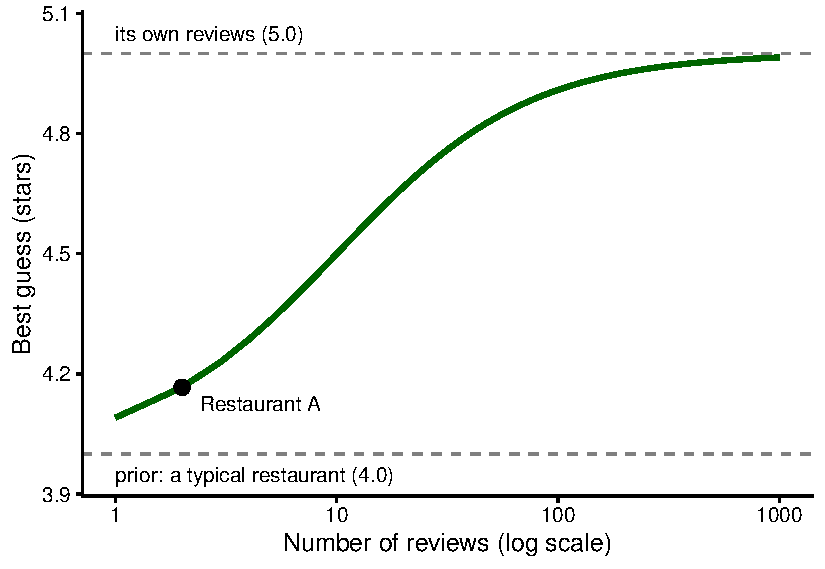
\includegraphics[keepaspectratio]{BSTA374_Lecture_BayesINLA_files/figure-pdf/fig-restaurants-1.pdf}}

}

\caption{\label{fig-restaurants}Best guess for a restaurant whose
reviews all give 5.0 stars, as reviews accumulate.}

\end{figure}%

With 2 reviews, the guess stays close to the prior. With 10 own reviews,
as many as the borrowed ones, it sits exactly halfway. With hundreds,
the prior hardly matters.

\begin{tcolorbox}[enhanced jigsaw, colbacktitle=quarto-callout-tip-color!10!white, leftrule=.75mm, colframe=quarto-callout-tip-color-frame, bottomrule=.15mm, left=2mm, titlerule=0mm, title=\textcolor{quarto-callout-tip-color}{\faLightbulb}\hspace{0.5em}{Key idea}, rightrule=.15mm, bottomtitle=1mm, colback=white, toptitle=1mm, coltitle=black, arc=.35mm, breakable, toprule=.15mm, opacitybacktitle=0.6, opacityback=0]

The posterior is a compromise between the prior and the data. The more
data, the more the data win.

\end{tcolorbox}

\section{Learning one test at a time: is the well water
safe?}\label{learning-one-test-at-a-time-is-the-well-water-safe}

\subsection{The story}\label{the-story}

A family tests its well for arsenic ten times. The EPA limit is 10 µg/L.
Their question: \textbf{how often is this water above the limit?} Call
that share \(\theta\): \(\theta = 0.2\) means unsafe one test in five.

\begin{Shaded}
\begin{Highlighting}[]
\NormalTok{epa   }\OtherTok{\textless{}{-}} \DecValTok{10}                                          \CommentTok{\# EPA limit, µg/L}
\NormalTok{conc  }\OtherTok{\textless{}{-}} \FunctionTok{c}\NormalTok{(}\DecValTok{14}\NormalTok{, }\DecValTok{7}\NormalTok{, }\DecValTok{12}\NormalTok{, }\DecValTok{18}\NormalTok{, }\DecValTok{11}\NormalTok{, }\DecValTok{15}\NormalTok{, }\DecValTok{9}\NormalTok{, }\DecValTok{13}\NormalTok{, }\DecValTok{14}\NormalTok{, }\DecValTok{14}\NormalTok{)     }\CommentTok{\# 10 tests (illustrative)}
\NormalTok{above }\OtherTok{\textless{}{-}} \FunctionTok{as.integer}\NormalTok{(conc }\SpecialCharTok{\textgreater{}}\NormalTok{ epa)                      }\CommentTok{\# 1 = above, 0 = below}
\NormalTok{above}
\end{Highlighting}
\end{Shaded}

\begin{verbatim}
 [1] 1 0 1 1 1 1 0 1 1 1
\end{verbatim}

We do not start from nothing. In nearby wells, about \textbf{half} of
past tests were above the limit: 5 of 10. That is our \textbf{prior},
centred on \(\theta = 0.5\). A Beta curve keeps the score: Beta(5, 5)
means 10 tests borrowed from the neighbours, 5 above and 5 below. Each
new test above the limit adds 1 to the first number, each test below
adds 1 to the second.

\subsection{Watching the posterior
learn}\label{watching-the-posterior-learn}

In each panel, red dotted is what we believed \textbf{before} the test,
green is what we believe \textbf{after}.

\begin{Shaded}
\begin{Highlighting}[]
\NormalTok{plot\_update }\OtherTok{\textless{}{-}} \ControlFlowTok{function}\NormalTok{(a, b, x, n, }\AttributeTok{title =} \StringTok{""}\NormalTok{) \{}
\NormalTok{  theta }\OtherTok{\textless{}{-}} \FunctionTok{seq}\NormalTok{(}\DecValTok{0}\NormalTok{, }\DecValTok{1}\NormalTok{, }\FloatTok{0.001}\NormalTok{)}
  \FunctionTok{plot}\NormalTok{(theta, }\FunctionTok{dbeta}\NormalTok{(theta, a, b), }\AttributeTok{type =} \StringTok{"l"}\NormalTok{, }\AttributeTok{lty =} \DecValTok{3}\NormalTok{, }\AttributeTok{lwd =} \DecValTok{3}\NormalTok{, }\AttributeTok{col =} \StringTok{"red"}\NormalTok{,}
       \AttributeTok{ylim =} \FunctionTok{c}\NormalTok{(}\DecValTok{0}\NormalTok{, }\DecValTok{4}\NormalTok{), }\AttributeTok{bty =} \StringTok{"l"}\NormalTok{, }\AttributeTok{xlab =} \FunctionTok{expression}\NormalTok{(theta), }\AttributeTok{ylab =} \StringTok{""}\NormalTok{,}
       \AttributeTok{main =}\NormalTok{ title)                                            }\CommentTok{\# before}
  \ControlFlowTok{if}\NormalTok{ (n }\SpecialCharTok{\textgreater{}} \DecValTok{0}\NormalTok{)                                                    }\CommentTok{\# no test, no update}
    \FunctionTok{lines}\NormalTok{(theta, }\FunctionTok{dbeta}\NormalTok{(theta, a }\SpecialCharTok{+}\NormalTok{ x, b }\SpecialCharTok{+}\NormalTok{ n }\SpecialCharTok{{-}}\NormalTok{ x), }\AttributeTok{lwd =} \DecValTok{3}\NormalTok{, }\AttributeTok{col =} \StringTok{"darkgreen"}\NormalTok{)  }\CommentTok{\# after}
\NormalTok{\}}
\end{Highlighting}
\end{Shaded}

\begin{Shaded}
\begin{Highlighting}[]
\FunctionTok{par}\NormalTok{(}\AttributeTok{mfrow =} \FunctionTok{c}\NormalTok{(}\DecValTok{3}\NormalTok{, }\DecValTok{4}\NormalTok{), }\AttributeTok{mar =} \FunctionTok{c}\NormalTok{(}\DecValTok{4}\NormalTok{, }\DecValTok{2}\NormalTok{, }\DecValTok{2}\NormalTok{, }\DecValTok{1}\NormalTok{))}

\NormalTok{a }\OtherTok{\textless{}{-}} \DecValTok{5}\NormalTok{; b }\OtherTok{\textless{}{-}} \DecValTok{5}                                      \CommentTok{\# prior: 5 of 10 above in nearby wells}
\FunctionTok{plot\_update}\NormalTok{(a, b, }\DecValTok{0}\NormalTok{, }\DecValTok{0}\NormalTok{, }\AttributeTok{title =} \StringTok{"Before testing: nearby wells"}\NormalTok{)}

\ControlFlowTok{for}\NormalTok{ (i }\ControlFlowTok{in} \DecValTok{1}\SpecialCharTok{:}\DecValTok{10}\NormalTok{) \{}
  \FunctionTok{plot\_update}\NormalTok{(a, b, above[i], }\DecValTok{1}\NormalTok{,}
              \AttributeTok{title =} \FunctionTok{paste0}\NormalTok{(}\StringTok{"\#"}\NormalTok{, i, }\StringTok{": "}\NormalTok{, conc[i], }\StringTok{" ug/L"}\NormalTok{,}
                             \FunctionTok{ifelse}\NormalTok{(above[i] }\SpecialCharTok{==} \DecValTok{1}\NormalTok{, }\StringTok{" (above)"}\NormalTok{, }\StringTok{" (below)"}\NormalTok{)))}
\NormalTok{  a }\OtherTok{\textless{}{-}}\NormalTok{ a }\SpecialCharTok{+}\NormalTok{ above[i]                                 }\CommentTok{\# after ...}
\NormalTok{  b }\OtherTok{\textless{}{-}}\NormalTok{ b }\SpecialCharTok{+} \DecValTok{1} \SpecialCharTok{{-}}\NormalTok{ above[i]                             }\CommentTok{\# ... becomes next before}
\NormalTok{\}}
\end{Highlighting}
\end{Shaded}

\begin{figure}[H]

\centering{

\pandocbounded{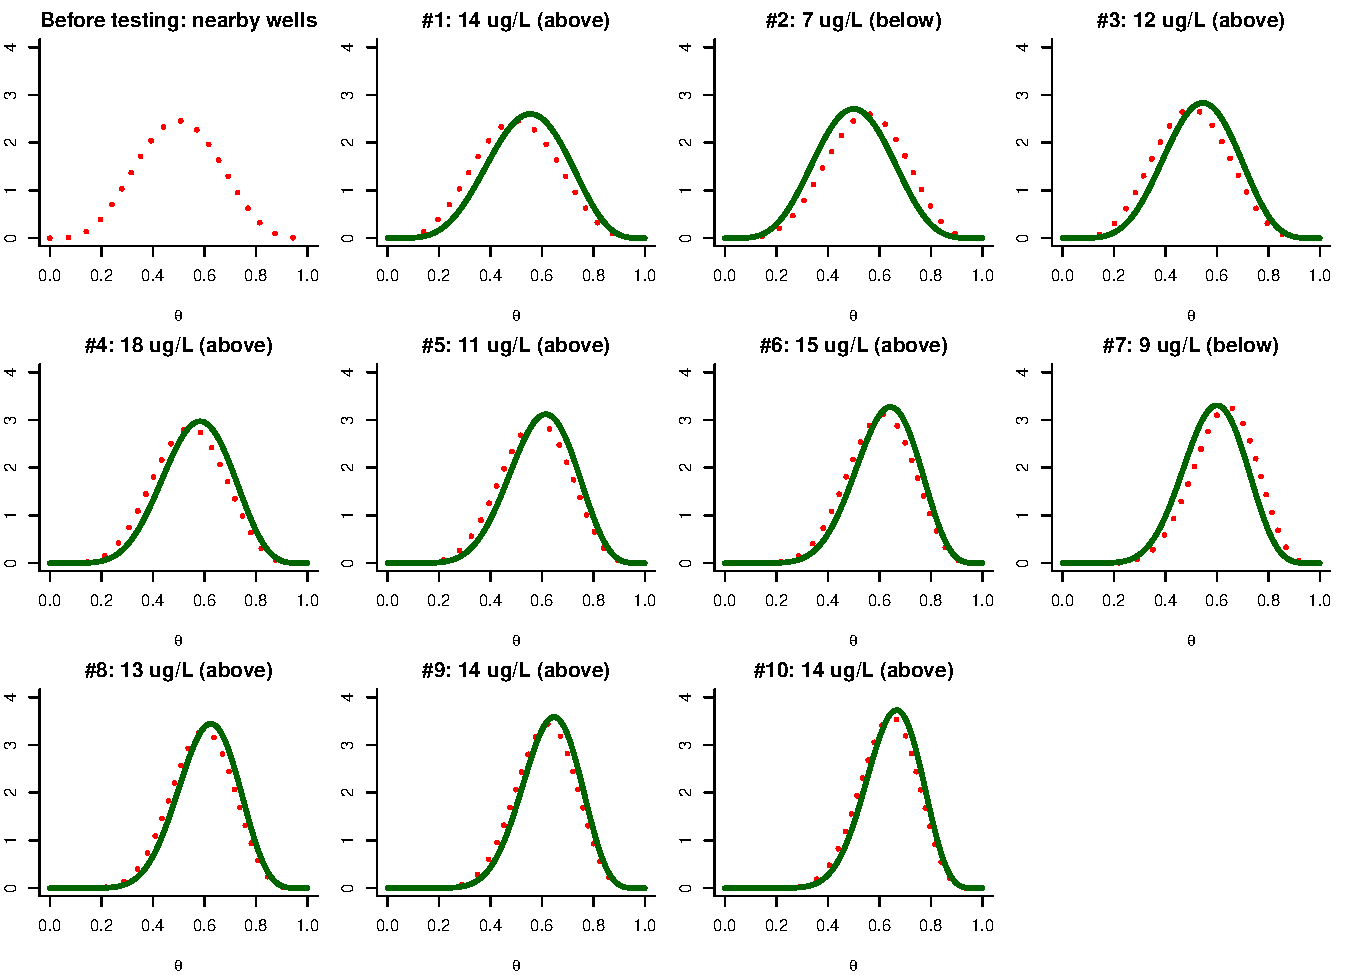
\includegraphics[keepaspectratio]{BSTA374_Lecture_BayesINLA_files/figure-pdf/fig-seq-chain-1.pdf}}

}

\caption{\label{fig-seq-chain}Each panel starts from the previous
panel's green curve and adds one test.}

\end{figure}%

Three things to notice:

\begin{enumerate}
\def\labelenumi{\arabic{enumi}.}
\tightlist
\item
  A test above the limit pushes the curve right; a test below pushes it
  left (tests 2 and 7).
\item
  The curve gets \textbf{taller and narrower}: more tests, more
  certainty.
\item
  Each panel's green curve becomes the next panel's red curve. That is
  Bayesian learning.
\end{enumerate}

\begin{tcolorbox}[enhanced jigsaw, colbacktitle=quarto-callout-note-color!10!white, leftrule=.75mm, colframe=quarto-callout-note-color-frame, bottomrule=.15mm, left=2mm, titlerule=0mm, title=\textcolor{quarto-callout-note-color}{\faInfo}\hspace{0.5em}{Note}, rightrule=.15mm, bottomtitle=1mm, colback=white, toptitle=1mm, coltitle=black, arc=.35mm, breakable, toprule=.15mm, opacitybacktitle=0.6, opacityback=0]

\textbf{Why does the y-axis stop at 4?} It shows a density, not a
probability, so it can exceed 1; the area under each curve is 1. We fix
it at 4 so the panels can be compared.

\end{tcolorbox}

\subsection{What do we know after ten
tests?}\label{what-do-we-know-after-ten-tests}

\begin{Shaded}
\begin{Highlighting}[]
\NormalTok{a }\SpecialCharTok{/}\NormalTok{ (a }\SpecialCharTok{+}\NormalTok{ b)                                      }\CommentTok{\# best guess for θ}
\end{Highlighting}
\end{Shaded}

\begin{verbatim}
[1] 0.65
\end{verbatim}

\begin{Shaded}
\begin{Highlighting}[]
\FunctionTok{qbeta}\NormalTok{(}\FunctionTok{c}\NormalTok{(}\FloatTok{0.025}\NormalTok{, }\FloatTok{0.975}\NormalTok{), a, b)                     }\CommentTok{\# 95\% credible interval}
\end{Highlighting}
\end{Shaded}

\begin{verbatim}
[1] 0.4344984 0.8371141
\end{verbatim}

\begin{Shaded}
\begin{Highlighting}[]
\DecValTok{1} \SpecialCharTok{{-}} \FunctionTok{pbeta}\NormalTok{(}\FloatTok{0.5}\NormalTok{, a, b)                             }\CommentTok{\# P(unsafe more than half the time)}
\end{Highlighting}
\end{Shaded}

\begin{verbatim}
[1] 0.9164658
\end{verbatim}

Our best guess is that the water is above the limit about 65\% of the
time, and with 95\% probability between 43\% and 84\% (the
\textbf{credible interval}). The probability that it is unsafe more than
half the time is 0.92. Bayesian results answer the family's question
directly, as a probability.

Where does 65\% come from? The well's own tests say 8 of 10, 80\%. The
nearby wells say 50\%. The 10 borrowed tests and the well's own 10 count
equally, so the answer sits halfway. It is the restaurant formula again:

\[
0.65 \;=\; w \times 0.80
\;+\; (1 - w) \times 0.50,
\qquad w = \frac{10}{10 + 10} = 0.5.
\]

\begin{tcolorbox}[enhanced jigsaw, colbacktitle=quarto-callout-tip-color!10!white, leftrule=.75mm, colframe=quarto-callout-tip-color-frame, bottomrule=.15mm, left=2mm, titlerule=0mm, title=\textcolor{quarto-callout-tip-color}{\faLightbulb}\hspace{0.5em}{Key idea}, rightrule=.15mm, bottomtitle=1mm, colback=white, toptitle=1mm, coltitle=black, arc=.35mm, breakable, toprule=.15mm, opacitybacktitle=0.6, opacityback=0]

We start from what we already know, here the nearby wells, and each new
test updates it. More data, a narrower curve, more certainty.

\end{tcolorbox}

\section{Counties: why small counties need
help}\label{counties-why-small-counties-need-help}

\subsection{The data}\label{the-data}

We rebuild the Pennsylvania lung cancer counts from the SIR lecture:
\(O\) observed cases, \(E\) expected cases, and SIR \(= O/E\).

\begin{Shaded}
\begin{Highlighting}[]
\FunctionTok{data}\NormalTok{(pennLC)}
\NormalTok{d }\OtherTok{\textless{}{-}}\NormalTok{ pennLC}\SpecialCharTok{$}\NormalTok{data}

\NormalTok{ref }\OtherTok{\textless{}{-}}\NormalTok{ d }\SpecialCharTok{|\textgreater{}}
  \FunctionTok{group\_by}\NormalTok{(race, gender, age) }\SpecialCharTok{|\textgreater{}}
  \FunctionTok{summarise}\NormalTok{(}\AttributeTok{r =} \FunctionTok{sum}\NormalTok{(cases) }\SpecialCharTok{/} \FunctionTok{sum}\NormalTok{(population), }\AttributeTok{.groups =} \StringTok{"drop"}\NormalTok{)   }\CommentTok{\# reference rates}

\NormalTok{county }\OtherTok{\textless{}{-}}\NormalTok{ d }\SpecialCharTok{|\textgreater{}}
  \FunctionTok{left\_join}\NormalTok{(ref, }\AttributeTok{by =} \FunctionTok{c}\NormalTok{(}\StringTok{"race"}\NormalTok{, }\StringTok{"gender"}\NormalTok{, }\StringTok{"age"}\NormalTok{)) }\SpecialCharTok{|\textgreater{}}
  \FunctionTok{group\_by}\NormalTok{(county) }\SpecialCharTok{|\textgreater{}}
  \FunctionTok{summarise}\NormalTok{(}\AttributeTok{O =} \FunctionTok{sum}\NormalTok{(cases), }\AttributeTok{E =} \FunctionTok{sum}\NormalTok{(population }\SpecialCharTok{*}\NormalTok{ r), }\AttributeTok{.groups =} \StringTok{"drop"}\NormalTok{) }\SpecialCharTok{|\textgreater{}}
  \FunctionTok{mutate}\NormalTok{(}\AttributeTok{county =} \FunctionTok{as.character}\NormalTok{(county), }\AttributeTok{SIR =}\NormalTok{ O }\SpecialCharTok{/}\NormalTok{ E)}

\NormalTok{pa }\OtherTok{\textless{}{-}} \FunctionTok{st\_as\_sf}\NormalTok{(pennLC}\SpecialCharTok{$}\NormalTok{spatial.polygon) }\SpecialCharTok{|\textgreater{}}
  \FunctionTok{st\_set\_crs}\NormalTok{(}\DecValTok{4326}\NormalTok{) }\SpecialCharTok{|\textgreater{}}
  \FunctionTok{mutate}\NormalTok{(}\AttributeTok{county =} \FunctionTok{names}\NormalTok{(pennLC}\SpecialCharTok{$}\NormalTok{spatial.polygon)) }\SpecialCharTok{|\textgreater{}}
  \FunctionTok{st\_transform}\NormalTok{(}\DecValTok{5070}\NormalTok{) }\SpecialCharTok{|\textgreater{}}                                           \CommentTok{\# Albers}
  \FunctionTok{left\_join}\NormalTok{(county, }\AttributeTok{by =} \StringTok{"county"}\NormalTok{)}

\NormalTok{sir\_breaks }\OtherTok{\textless{}{-}} \FunctionTok{c}\NormalTok{(}\DecValTok{0}\NormalTok{, }\FloatTok{0.67}\NormalTok{, }\FloatTok{0.83}\NormalTok{, }\FloatTok{0.95}\NormalTok{, }\FloatTok{1.05}\NormalTok{, }\FloatTok{1.2}\NormalTok{, }\FloatTok{1.5}\NormalTok{, }\ConstantTok{Inf}\NormalTok{)}
\NormalTok{sir\_fill   }\OtherTok{\textless{}{-}} \FunctionTok{scale\_fill\_brewer}\NormalTok{(}\AttributeTok{palette =} \StringTok{"RdBu"}\NormalTok{, }\AttributeTok{direction =} \SpecialCharTok{{-}}\DecValTok{1}\NormalTok{, }\AttributeTok{drop =} \ConstantTok{FALSE}\NormalTok{, }\AttributeTok{name =} \StringTok{"Risk"}\NormalTok{)}
\end{Highlighting}
\end{Shaded}

\subsection{The SIR map}\label{the-sir-map}

\begin{Shaded}
\begin{Highlighting}[]
\FunctionTok{ggplot}\NormalTok{(pa) }\SpecialCharTok{+}
  \FunctionTok{geom\_sf}\NormalTok{(}\FunctionTok{aes}\NormalTok{(}\AttributeTok{fill =} \FunctionTok{cut}\NormalTok{(SIR, sir\_breaks)), }\AttributeTok{colour =} \StringTok{"white"}\NormalTok{, }\AttributeTok{linewidth =} \FloatTok{0.2}\NormalTok{) }\SpecialCharTok{+}
\NormalTok{  sir\_fill }\SpecialCharTok{+}
  \FunctionTok{theme\_void}\NormalTok{(}\AttributeTok{base\_size =} \DecValTok{12}\NormalTok{)}
\end{Highlighting}
\end{Shaded}

\begin{figure}[H]

\centering{

\pandocbounded{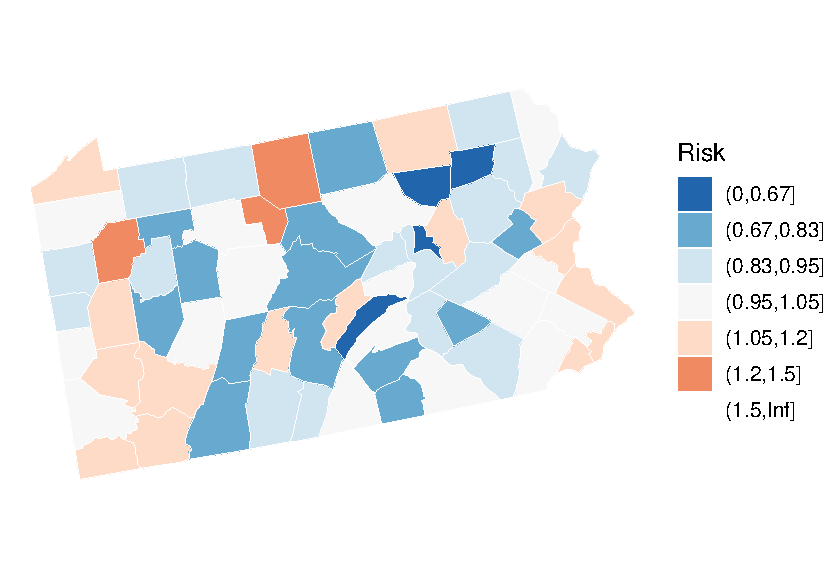
\includegraphics[keepaspectratio]{BSTA374_Lecture_BayesINLA_files/figure-pdf/fig-sir-1.pdf}}

}

\caption{\label{fig-sir}Lung cancer SIRs, Pennsylvania counties.}

\end{figure}%

Which counties have the most extreme SIRs?

\begin{Shaded}
\begin{Highlighting}[]
\NormalTok{extremes }\OtherTok{\textless{}{-}}\NormalTok{ county }\SpecialCharTok{|\textgreater{}}
  \FunctionTok{arrange}\NormalTok{(SIR) }\SpecialCharTok{|\textgreater{}}
  \FunctionTok{slice}\NormalTok{(}\FunctionTok{c}\NormalTok{(}\DecValTok{1}\SpecialCharTok{:}\DecValTok{3}\NormalTok{, }\DecValTok{65}\SpecialCharTok{:}\DecValTok{67}\NormalTok{)) }\SpecialCharTok{|\textgreater{}}                           \CommentTok{\# 3 lowest, 3 highest}
  \FunctionTok{mutate}\NormalTok{(}\AttributeTok{E =} \FunctionTok{round}\NormalTok{(E, }\DecValTok{1}\NormalTok{), }\AttributeTok{SIR =} \FunctionTok{round}\NormalTok{(SIR, }\DecValTok{2}\NormalTok{))}
\NormalTok{extremes}
\end{Highlighting}
\end{Shaded}

\begin{verbatim}
# A tibble: 6 x 4
  county       O     E   SIR
  <chr>    <int> <dbl> <dbl>
1 juniata      6  18.7  0.32
2 sullivan     3   7.4  0.4 
3 montour      8  16.1  0.5 
4 cameron      8   5.9  1.35
5 venango     70  51.1  1.37
6 potter      22  16    1.37
\end{verbatim}

Of these six counties, 5 expect fewer than 20 cases; the median county
expects 75. A few cases more or less move their SIR a lot. Small
counties are like restaurants with two reviews.

\subsection{The funnel plot}\label{the-funnel-plot}

How far can an SIR stray by chance alone? If a county's true risk were
exactly the state's, its SIR would still fall, about 95\% of the time,
within \(1 \pm 1.96/\sqrt{E}\). Plotted against \(E\), that range is a
funnel.

\begin{Shaded}
\begin{Highlighting}[]
\NormalTok{funnel }\OtherTok{\textless{}{-}} \FunctionTok{tibble}\NormalTok{(}\AttributeTok{E =} \FunctionTok{exp}\NormalTok{(}\FunctionTok{seq}\NormalTok{(}\FunctionTok{log}\NormalTok{(}\DecValTok{4}\NormalTok{), }\FunctionTok{log}\NormalTok{(}\DecValTok{1500}\NormalTok{), }\AttributeTok{length.out =} \DecValTok{200}\NormalTok{))) }\SpecialCharTok{|\textgreater{}}
  \FunctionTok{mutate}\NormalTok{(}\AttributeTok{lo =} \DecValTok{1} \SpecialCharTok{{-}} \FloatTok{1.96} \SpecialCharTok{/} \FunctionTok{sqrt}\NormalTok{(E),                   }\CommentTok{\# chance range of the SIR}
         \AttributeTok{hi =} \DecValTok{1} \SpecialCharTok{+} \FloatTok{1.96} \SpecialCharTok{/} \FunctionTok{sqrt}\NormalTok{(E))}

\NormalTok{labelled }\OtherTok{\textless{}{-}} \FunctionTok{filter}\NormalTok{(county, county }\SpecialCharTok{\%in\%} \FunctionTok{c}\NormalTok{(}\StringTok{"sullivan"}\NormalTok{, }\StringTok{"potter"}\NormalTok{, }\StringTok{"juniata"}\NormalTok{, }\StringTok{"philadelphia"}\NormalTok{))}

\FunctionTok{ggplot}\NormalTok{() }\SpecialCharTok{+}
  \FunctionTok{geom\_ribbon}\NormalTok{(}\AttributeTok{data =}\NormalTok{ funnel, }\FunctionTok{aes}\NormalTok{(E, }\AttributeTok{ymin =}\NormalTok{ lo, }\AttributeTok{ymax =}\NormalTok{ hi), }\AttributeTok{fill =} \StringTok{"grey85"}\NormalTok{) }\SpecialCharTok{+}
  \FunctionTok{geom\_hline}\NormalTok{(}\AttributeTok{yintercept =} \DecValTok{1}\NormalTok{, }\AttributeTok{colour =} \StringTok{"grey50"}\NormalTok{) }\SpecialCharTok{+}
  \FunctionTok{geom\_point}\NormalTok{(}\AttributeTok{data =}\NormalTok{ county, }\FunctionTok{aes}\NormalTok{(E, SIR)) }\SpecialCharTok{+}
  \FunctionTok{geom\_text}\NormalTok{(}\AttributeTok{data =}\NormalTok{ labelled, }\FunctionTok{aes}\NormalTok{(E, SIR, }\AttributeTok{label =}\NormalTok{ tools}\SpecialCharTok{::}\FunctionTok{toTitleCase}\NormalTok{(county)),}
            \AttributeTok{nudge\_y =} \FloatTok{0.07}\NormalTok{, }\AttributeTok{size =} \FloatTok{3.5}\NormalTok{) }\SpecialCharTok{+}
  \FunctionTok{scale\_x\_log10}\NormalTok{() }\SpecialCharTok{+}
  \FunctionTok{labs}\NormalTok{(}\AttributeTok{x =} \StringTok{"Expected cases (log scale)"}\NormalTok{, }\AttributeTok{y =} \StringTok{"SIR"}\NormalTok{) }\SpecialCharTok{+}
  \FunctionTok{theme\_classic}\NormalTok{(}\AttributeTok{base\_size =} \DecValTok{12}\NormalTok{)}
\end{Highlighting}
\end{Shaded}

\begin{figure}[H]

\centering{

\pandocbounded{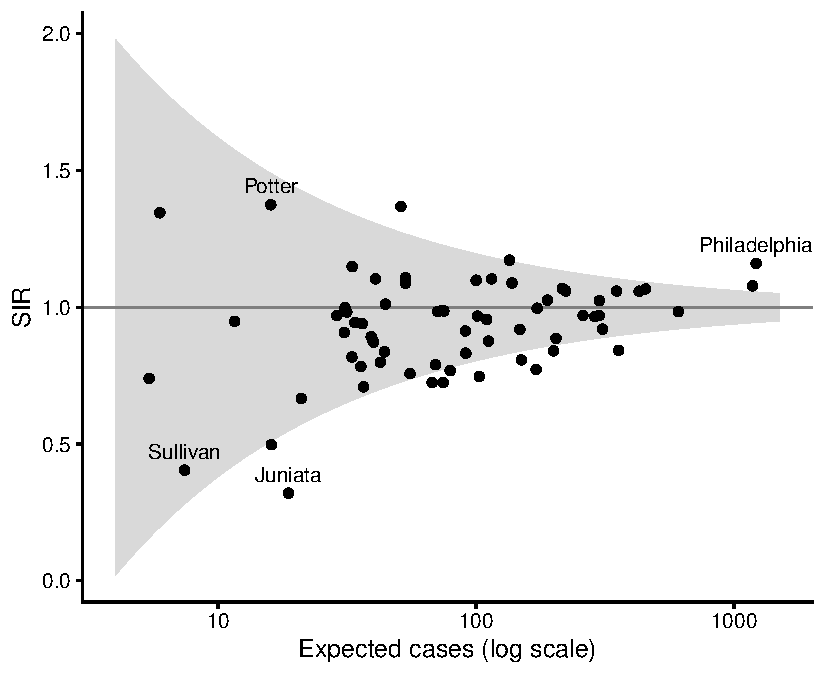
\includegraphics[keepaspectratio]{BSTA374_Lecture_BayesINLA_files/figure-pdf/fig-funnel-1.pdf}}

}

\caption{\label{fig-funnel}SIRs against expected cases. Grey: where
about 95\% of SIRs fall by chance alone.}

\end{figure}%

The funnel is wide on the left. Potter's 1.37 and Sullivan's 0.40 sit
inside it: they could be chance. Philadelphia's 1.16 is far outside:
with more than 1,200 expected cases, a 16\% excess is not chance.

\begin{tcolorbox}[enhanced jigsaw, colbacktitle=quarto-callout-important-color!10!white, leftrule=.75mm, colframe=quarto-callout-important-color-frame, bottomrule=.15mm, left=2mm, titlerule=0mm, title=\textcolor{quarto-callout-important-color}{\faExclamation}\hspace{0.5em}{The problem in one sentence}, rightrule=.15mm, bottomtitle=1mm, colback=white, toptitle=1mm, coltitle=black, arc=.35mm, breakable, toprule=.15mm, opacitybacktitle=0.6, opacityback=0]

A raw SIR mixes real differences in risk with chance, and chance is
largest in small counties.

\end{tcolorbox}

\section{Shrinkage: the restaurant formula for
counties}\label{shrinkage-the-restaurant-formula-for-counties}

\subsection{Same formula, new names}\label{same-formula-new-names}

\begin{longtable}[]{@{}
  >{\raggedright\arraybackslash}p{(\linewidth - 2\tabcolsep) * \real{0.5000}}
  >{\raggedright\arraybackslash}p{(\linewidth - 2\tabcolsep) * \real{0.5000}}@{}}
\toprule\noalign{}
\begin{minipage}[b]{\linewidth}\raggedright
Restaurants
\end{minipage} & \begin{minipage}[b]{\linewidth}\raggedright
Counties
\end{minipage} \\
\midrule\noalign{}
\endhead
\bottomrule\noalign{}
\endlastfoot
number of reviews & expected cases \(E\) \\
its average rating & its SIR \\
a typical restaurant, 4.0 & the state average, 1 \\
10 borrowed ratings, average 4.0 & \(k\) borrowed expected cases at the
state rate \\
trust in its own reviews, \(w\) & trust in its own SIR, \(w\) \\
\end{longtable}

So each county gets

\[
\text{estimate} \;=\; w \times \text{SIR} \;+\; (1 - w) \times 1,
\qquad w = \frac{E}{E + k}.
\]

A big county (large \(E\)) keeps its SIR. A small county borrows from
the state.

\subsection{\texorpdfstring{Who decides \(k\)? The
data}{Who decides k? The data}}\label{who-decides-k-the-data}

For the restaurants we picked 10 ourselves. For counties, R estimates
\(k\) from the 67 SIRs:

\begin{itemize}
\tightlist
\item
  if counties differ \textbf{much more} than chance alone would produce,
  real differences are large, we trust each county's SIR, and \(k\) is
  small;
\item
  if counties differ \textbf{about as much} as chance would produce, we
  trust the state average more, and \(k\) is large.
\end{itemize}

Letting the data choose the prior this way is called \textbf{empirical
Bayes} (Clayton and Kaldor 1987; Marshall 1991). \texttt{EBest()} in
\textbf{spdep} does it in one line.

\begin{Shaded}
\begin{Highlighting}[]
\NormalTok{eb }\OtherTok{\textless{}{-}} \FunctionTok{EBest}\NormalTok{(pa}\SpecialCharTok{$}\NormalTok{O, pa}\SpecialCharTok{$}\NormalTok{E)                              }\CommentTok{\# cases, expected cases}
\NormalTok{pa}\SpecialCharTok{$}\NormalTok{RR\_eb }\OtherTok{\textless{}{-}}\NormalTok{ eb}\SpecialCharTok{$}\NormalTok{estmm                                 }\CommentTok{\# shrunk estimate}

\NormalTok{k }\OtherTok{\textless{}{-}} \FunctionTok{with}\NormalTok{(}\FunctionTok{attr}\NormalTok{(eb, }\StringTok{"parameters"}\NormalTok{), b }\SpecialCharTok{/}\NormalTok{ a)             }\CommentTok{\# k borrowed expected cases}
\NormalTok{k}
\end{Highlighting}
\end{Shaded}

\begin{verbatim}
[1] 107.908
\end{verbatim}

\begin{Shaded}
\begin{Highlighting}[]
\NormalTok{pa}\SpecialCharTok{$}\NormalTok{w }\OtherTok{\textless{}{-}}\NormalTok{ pa}\SpecialCharTok{$}\NormalTok{E }\SpecialCharTok{/}\NormalTok{ (pa}\SpecialCharTok{$}\NormalTok{E }\SpecialCharTok{+}\NormalTok{ k)                            }\CommentTok{\# trust in own SIR}
\end{Highlighting}
\end{Shaded}

Each county borrows about 108 expected cases at the state rate. Here are
five counties, from small to large:

\begin{Shaded}
\begin{Highlighting}[]
\NormalTok{pa }\SpecialCharTok{|\textgreater{}}
  \FunctionTok{st\_drop\_geometry}\NormalTok{() }\SpecialCharTok{|\textgreater{}}
  \FunctionTok{filter}\NormalTok{(county }\SpecialCharTok{\%in\%} \FunctionTok{c}\NormalTok{(}\StringTok{"sullivan"}\NormalTok{, }\StringTok{"potter"}\NormalTok{, }\StringTok{"venango"}\NormalTok{, }\StringTok{"lehigh"}\NormalTok{, }\StringTok{"philadelphia"}\NormalTok{)) }\SpecialCharTok{|\textgreater{}}
  \FunctionTok{arrange}\NormalTok{(E) }\SpecialCharTok{|\textgreater{}}
  \FunctionTok{transmute}\NormalTok{(county, }\AttributeTok{E =} \FunctionTok{round}\NormalTok{(E), }\AttributeTok{SIR =} \FunctionTok{round}\NormalTok{(SIR, }\DecValTok{2}\NormalTok{),}
            \AttributeTok{w =} \FunctionTok{round}\NormalTok{(w, }\DecValTok{2}\NormalTok{), }\AttributeTok{estimate =} \FunctionTok{round}\NormalTok{(RR\_eb, }\DecValTok{2}\NormalTok{))}
\end{Highlighting}
\end{Shaded}

\begin{verbatim}
        county    E  SIR    w estimate
1     sullivan    7 0.40 0.06     0.96
2       potter   16 1.37 0.13     1.05
3      venango   51 1.37 0.32     1.12
4       lehigh  260 0.97 0.71     0.98
5 philadelphia 1219 1.16 0.92     1.15
\end{verbatim}

Sullivan's own 7 expected cases are mixed with 108 borrowed ones: we
trust its SIR only 6\%, and its estimate is almost the state's.
Philadelphia, with more than 1,200 expected cases, keeps 92\% of its
SIR. Potter and Venango have the same SIR, 1.37, like two restaurants
with the same average, but Venango rests on three times more cases, so
it stays higher: 1.12 against 1.05.

\subsection{Where do we borrow?}\label{where-do-we-borrow}

\begin{Shaded}
\begin{Highlighting}[]
\FunctionTok{ggplot}\NormalTok{(pa) }\SpecialCharTok{+}
  \FunctionTok{geom\_sf}\NormalTok{(}\FunctionTok{aes}\NormalTok{(}\AttributeTok{fill =}\NormalTok{ w), }\AttributeTok{colour =} \StringTok{"white"}\NormalTok{, }\AttributeTok{linewidth =} \FloatTok{0.2}\NormalTok{) }\SpecialCharTok{+}
  \FunctionTok{scale\_fill\_distiller}\NormalTok{(}\AttributeTok{palette =} \StringTok{"Purples"}\NormalTok{, }\AttributeTok{direction =} \DecValTok{1}\NormalTok{, }\AttributeTok{limits =} \FunctionTok{c}\NormalTok{(}\DecValTok{0}\NormalTok{, }\DecValTok{1}\NormalTok{),}
                       \AttributeTok{name =} \StringTok{"Trust w"}\NormalTok{) }\SpecialCharTok{+}
  \FunctionTok{theme\_void}\NormalTok{(}\AttributeTok{base\_size =} \DecValTok{12}\NormalTok{)}
\end{Highlighting}
\end{Shaded}

\begin{figure}[H]

\centering{

\pandocbounded{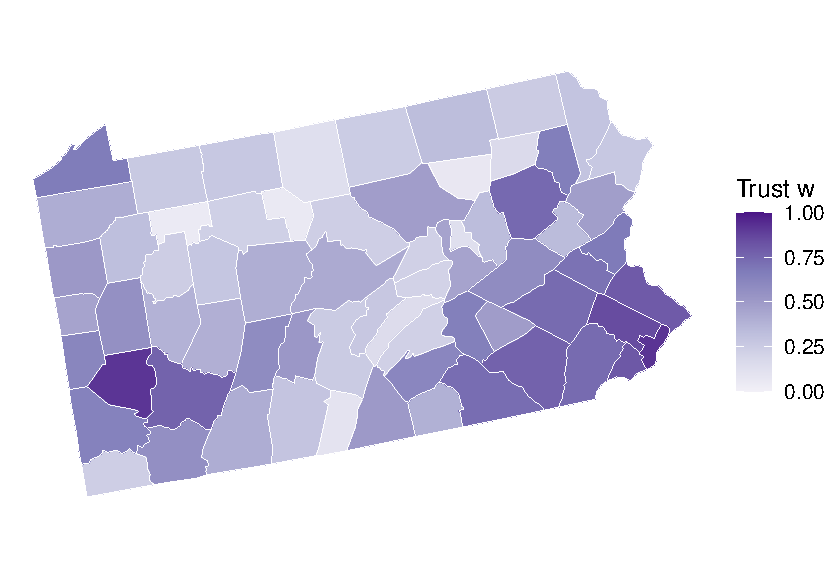
\includegraphics[keepaspectratio]{BSTA374_Lecture_BayesINLA_files/figure-pdf/fig-weights-1.pdf}}

}

\caption{\label{fig-weights}Trust in each county's own SIR. Dark: we
keep the county's SIR. Light: we borrow from the state.}

\end{figure}%

The map of \(w\) is a map of population: the rural north and centre
borrow the most, the Philadelphia and Pittsburgh areas the least.

\begin{tcolorbox}[enhanced jigsaw, colbacktitle=quarto-callout-tip-color!10!white, leftrule=.75mm, colframe=quarto-callout-tip-color-frame, bottomrule=.15mm, left=2mm, titlerule=0mm, title=\textcolor{quarto-callout-tip-color}{\faLightbulb}\hspace{0.5em}{Key idea}, rightrule=.15mm, bottomtitle=1mm, colback=white, toptitle=1mm, coltitle=black, arc=.35mm, breakable, toprule=.15mm, opacitybacktitle=0.6, opacityback=0]

Small counties borrow from the state; big counties keep their own SIR.
The data decide how much to borrow.

\end{tcolorbox}

\section{Full Bayes with R-INLA}\label{full-bayes-with-r-inla}

Empirical Bayes gives one number per county. A \textbf{full Bayesian}
model does the same shrinkage but returns a whole posterior curve per
county, like the green curves of the well. That tells us \textbf{how
sure} we are. INLA is a fast way to fit such models (Moraga Ch. 3--4).

We use the \textbf{BYM2} model (Moraga §5.3). Instead of borrowing from
the whole state, each county borrows mostly from its
\textbf{neighbours}, the way the family borrowed from nearby wells. We
use the queen neighbours from the Moran's I lecture.

\begin{Shaded}
\begin{Highlighting}[]
\NormalTok{dat }\OtherTok{\textless{}{-}} \FunctionTok{st\_drop\_geometry}\NormalTok{(pa) }\SpecialCharTok{|\textgreater{}}
  \FunctionTok{mutate}\NormalTok{(}\AttributeTok{id =} \FunctionTok{row\_number}\NormalTok{())                          }\CommentTok{\# one index per county}

\NormalTok{nb }\OtherTok{\textless{}{-}} \FunctionTok{poly2nb}\NormalTok{(pa, }\AttributeTok{queen =} \ConstantTok{TRUE}\NormalTok{)                      }\CommentTok{\# queen neighbours}
\FunctionTok{nb2INLA}\NormalTok{(}\StringTok{"pa.adj"}\NormalTok{, nb)                                }\CommentTok{\# write for INLA}
\NormalTok{g  }\OtherTok{\textless{}{-}} \FunctionTok{inla.read.graph}\NormalTok{(}\StringTok{"pa.adj"}\NormalTok{)}

\NormalTok{m2 }\OtherTok{\textless{}{-}} \FunctionTok{inla}\NormalTok{(O }\SpecialCharTok{\textasciitilde{}} \DecValTok{1} \SpecialCharTok{+} \FunctionTok{f}\NormalTok{(id, }\AttributeTok{model =} \StringTok{"bym2"}\NormalTok{, }\AttributeTok{graph =}\NormalTok{ g),}
           \AttributeTok{family =} \StringTok{"poisson"}\NormalTok{, }\AttributeTok{E =}\NormalTok{ E, }\AttributeTok{data =}\NormalTok{ dat,}
           \AttributeTok{control.predictor =} \FunctionTok{list}\NormalTok{(}\AttributeTok{compute =} \ConstantTok{TRUE}\NormalTok{),}
           \AttributeTok{control.compute =} \FunctionTok{list}\NormalTok{(}\AttributeTok{return.marginals.predictor =} \ConstantTok{TRUE}\NormalTok{))}

\NormalTok{dat}\SpecialCharTok{$}\NormalTok{RR\_bym2 }\OtherTok{\textless{}{-}}\NormalTok{ m2}\SpecialCharTok{$}\NormalTok{summary.fitted.values}\SpecialCharTok{$}\NormalTok{mean         }\CommentTok{\# posterior mean risk}
\end{Highlighting}
\end{Shaded}

Read the formula as: log-risk = an overall level + a bump for each
county that borrows from its neighbours (Moraga §4.1).

\subsection{How does INLA get a credible
interval?}\label{how-does-inla-get-a-credible-interval}

For every county, INLA returns a whole \textbf{posterior curve} for its
relative risk, like the green curves of the well. For the well, a simple
formula gave the curve. Here it cannot, because each county borrows from
its neighbours, and we do not know \textbf{how much} to borrow: that
depends on how different the counties really are, which is itself
unknown. INLA works in three steps (Moraga §3.2):

\begin{enumerate}
\def\labelenumi{\arabic{enumi}.}
\tightlist
\item
  \textbf{Try several amounts of borrowing.} For each plausible value of
  how much the counties differ, it computes the county's curve with a
  fast bell-shaped (Laplace) approximation.
\item
  \textbf{Average the curves.} It weights each curve by how well that
  amount of borrowing fits all 67 counties, and averages them. This is
  the \emph{integrated} in INLA.
\item
  \textbf{Read the final curve.} The posterior mean is its balance
  point; the 95\% credible interval cuts 2.5\% of the area off each
  side; the exceedance probability is the area to the right of 1.
\end{enumerate}

Here are steps 1 and 2 for Potter. Each dashed curve fixes one amount of
borrowing, from little to a lot; the thick grey curve is INLA's final
curve.

\begin{Shaded}
\begin{Highlighting}[]
\NormalTok{k   }\OtherTok{\textless{}{-}} \FunctionTok{which}\NormalTok{(dat}\SpecialCharTok{$}\NormalTok{county }\SpecialCharTok{==} \StringTok{"potter"}\NormalTok{)}
\NormalTok{tau }\OtherTok{\textless{}{-}} \FunctionTok{c}\NormalTok{(}\DecValTok{10}\NormalTok{, m2}\SpecialCharTok{$}\NormalTok{summary.hyperpar[}\StringTok{"Precision for id"}\NormalTok{, }\StringTok{"0.5quant"}\NormalTok{], }\DecValTok{1000}\NormalTok{)   }\CommentTok{\# little, middle, a lot}
\NormalTok{phi }\OtherTok{\textless{}{-}}\NormalTok{ m2}\SpecialCharTok{$}\NormalTok{summary.hyperpar[}\StringTok{"Phi for id"}\NormalTok{, }\StringTok{"0.5quant"}\NormalTok{]}

\NormalTok{fixed\_fit }\OtherTok{\textless{}{-}} \ControlFlowTok{function}\NormalTok{(t) \{                           }\CommentTok{\# BYM2 with borrowing fixed}
\NormalTok{  hyp }\OtherTok{\textless{}{-}} \FunctionTok{list}\NormalTok{(}\AttributeTok{prec =} \FunctionTok{list}\NormalTok{(}\AttributeTok{initial =} \FunctionTok{log}\NormalTok{(t),   }\AttributeTok{fixed =} \ConstantTok{TRUE}\NormalTok{),}
              \AttributeTok{phi  =} \FunctionTok{list}\NormalTok{(}\AttributeTok{initial =} \FunctionTok{qlogis}\NormalTok{(phi), }\AttributeTok{fixed =} \ConstantTok{TRUE}\NormalTok{))}
\NormalTok{  m }\OtherTok{\textless{}{-}} \FunctionTok{inla}\NormalTok{(O }\SpecialCharTok{\textasciitilde{}} \DecValTok{1} \SpecialCharTok{+} \FunctionTok{f}\NormalTok{(id, }\AttributeTok{model =} \StringTok{"bym2"}\NormalTok{, }\AttributeTok{graph =}\NormalTok{ g, }\AttributeTok{hyper =}\NormalTok{ hyp),}
            \AttributeTok{family =} \StringTok{"poisson"}\NormalTok{, }\AttributeTok{E =}\NormalTok{ E, }\AttributeTok{data =}\NormalTok{ dat,}
            \AttributeTok{control.predictor =} \FunctionTok{list}\NormalTok{(}\AttributeTok{compute =} \ConstantTok{TRUE}\NormalTok{),}
            \AttributeTok{control.compute =} \FunctionTok{list}\NormalTok{(}\AttributeTok{return.marginals.predictor =} \ConstantTok{TRUE}\NormalTok{))}
  \FunctionTok{inla.smarginal}\NormalTok{(m}\SpecialCharTok{$}\NormalTok{marginals.fitted.values[[k]])     }\CommentTok{\# Potter\textquotesingle{}s curve}
\NormalTok{\}}

\NormalTok{lab }\OtherTok{\textless{}{-}} \FunctionTok{c}\NormalTok{(}\StringTok{"borrow little (counties very different)"}\NormalTok{, }\StringTok{"borrow a middle amount"}\NormalTok{,}
         \StringTok{"borrow a lot (counties very similar)"}\NormalTok{)}
\NormalTok{steps }\OtherTok{\textless{}{-}} \FunctionTok{bind\_rows}\NormalTok{(}\FunctionTok{lapply}\NormalTok{(}\DecValTok{1}\SpecialCharTok{:}\DecValTok{3}\NormalTok{, }\ControlFlowTok{function}\NormalTok{(j) }\FunctionTok{data.frame}\NormalTok{(}\FunctionTok{fixed\_fit}\NormalTok{(tau[j]), }\AttributeTok{curve =}\NormalTok{ lab[j]))) }\SpecialCharTok{|\textgreater{}}
  \FunctionTok{mutate}\NormalTok{(}\AttributeTok{curve =} \FunctionTok{factor}\NormalTok{(curve, lab))}
\NormalTok{final }\OtherTok{\textless{}{-}} \FunctionTok{data.frame}\NormalTok{(}\FunctionTok{inla.smarginal}\NormalTok{(m2}\SpecialCharTok{$}\NormalTok{marginals.fitted.values[[k]]))}

\FunctionTok{ggplot}\NormalTok{() }\SpecialCharTok{+}
  \FunctionTok{geom\_line}\NormalTok{(}\AttributeTok{data =}\NormalTok{ final, }\FunctionTok{aes}\NormalTok{(x, y), }\AttributeTok{linewidth =} \FloatTok{2.5}\NormalTok{, }\AttributeTok{alpha =} \FloatTok{0.35}\NormalTok{) }\SpecialCharTok{+}     \CommentTok{\# final curve, underneath}
  \FunctionTok{geom\_line}\NormalTok{(}\AttributeTok{data =}\NormalTok{ steps, }\FunctionTok{aes}\NormalTok{(x, y, }\AttributeTok{colour =}\NormalTok{ curve), }\AttributeTok{linetype =} \DecValTok{2}\NormalTok{, }\AttributeTok{linewidth =} \FloatTok{0.9}\NormalTok{) }\SpecialCharTok{+}
  \FunctionTok{geom\_vline}\NormalTok{(}\AttributeTok{xintercept =}\NormalTok{ dat}\SpecialCharTok{$}\NormalTok{SIR[k], }\AttributeTok{linetype =} \DecValTok{3}\NormalTok{, }\AttributeTok{colour =} \StringTok{"blue"}\NormalTok{) }\SpecialCharTok{+}
  \FunctionTok{annotate}\NormalTok{(}\StringTok{"text"}\NormalTok{, }\AttributeTok{x =}\NormalTok{ dat}\SpecialCharTok{$}\NormalTok{SIR[k], }\AttributeTok{y =} \DecValTok{0}\NormalTok{, }\AttributeTok{label =} \StringTok{" Potter\textquotesingle{}s SIR"}\NormalTok{, }\AttributeTok{hjust =} \DecValTok{0}\NormalTok{,}
           \AttributeTok{vjust =} \SpecialCharTok{{-}}\FloatTok{0.5}\NormalTok{, }\AttributeTok{colour =} \StringTok{"blue"}\NormalTok{, }\AttributeTok{size =} \FloatTok{3.5}\NormalTok{) }\SpecialCharTok{+}
  \FunctionTok{scale\_colour\_manual}\NormalTok{(}\AttributeTok{values =} \FunctionTok{c}\NormalTok{(}\StringTok{"\#D95F02"}\NormalTok{, }\StringTok{"\#7570B3"}\NormalTok{, }\StringTok{"\#1B9E77"}\NormalTok{), }\AttributeTok{name =} \ConstantTok{NULL}\NormalTok{) }\SpecialCharTok{+}
  \FunctionTok{coord\_cartesian}\NormalTok{(}\AttributeTok{xlim =} \FunctionTok{c}\NormalTok{(}\FloatTok{0.5}\NormalTok{, }\FloatTok{1.8}\NormalTok{)) }\SpecialCharTok{+}
  \FunctionTok{labs}\NormalTok{(}\AttributeTok{x =} \StringTok{"Relative risk, Potter"}\NormalTok{, }\AttributeTok{y =} \StringTok{"Posterior density"}\NormalTok{) }\SpecialCharTok{+}
  \FunctionTok{theme\_classic}\NormalTok{(}\AttributeTok{base\_size =} \DecValTok{12}\NormalTok{) }\SpecialCharTok{+}
  \FunctionTok{theme}\NormalTok{(}\AttributeTok{legend.position =} \StringTok{"bottom"}\NormalTok{, }\AttributeTok{legend.direction =} \StringTok{"vertical"}\NormalTok{)}
\end{Highlighting}
\end{Shaded}

\begin{figure}[H]

\centering{

\pandocbounded{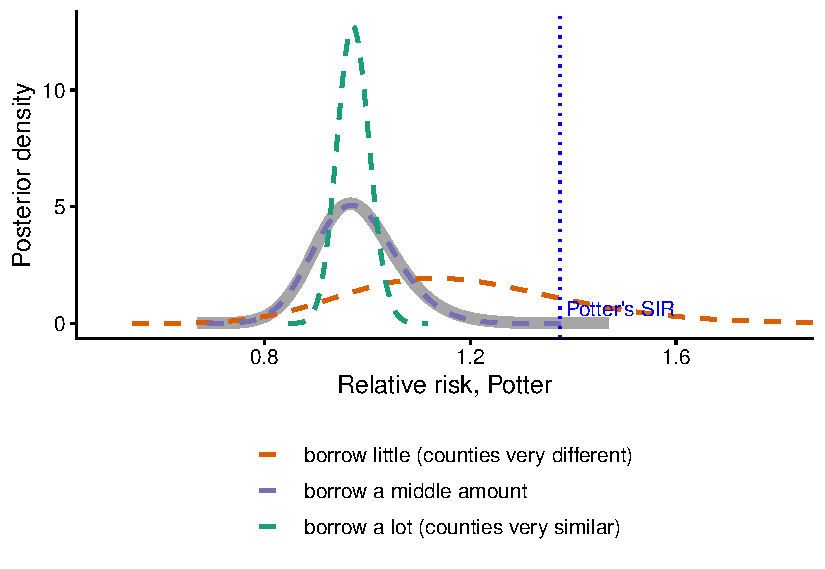
\includegraphics[keepaspectratio]{BSTA374_Lecture_BayesINLA_files/figure-pdf/fig-inla-steps-1.pdf}}

}

\caption{\label{fig-inla-steps}Potter County. Dashed: posterior curves
for three fixed amounts of borrowing. Thick grey: INLA's final curve,
which averages over all plausible amounts.}

\end{figure}%

Borrowing little leaves Potter closer to its own SIR, with a wide curve;
borrowing a lot pulls it toward its neighbours, with a narrow curve. The
data make the middle amount the most plausible, so the final curve sits
close to it. Step 3 then reads the answers off the final curve:

\begin{Shaded}
\begin{Highlighting}[]
\NormalTok{LL }\OtherTok{\textless{}{-}}\NormalTok{ m2}\SpecialCharTok{$}\NormalTok{summary.fitted.values}\SpecialCharTok{$}\StringTok{\textasciigrave{}}\AttributeTok{0.025quant}\StringTok{\textasciigrave{}}\NormalTok{[k]}
\NormalTok{UL }\OtherTok{\textless{}{-}}\NormalTok{ m2}\SpecialCharTok{$}\NormalTok{summary.fitted.values}\SpecialCharTok{$}\StringTok{\textasciigrave{}}\AttributeTok{0.975quant}\StringTok{\textasciigrave{}}\NormalTok{[k]}
\NormalTok{P1 }\OtherTok{\textless{}{-}} \DecValTok{1} \SpecialCharTok{{-}} \FunctionTok{inla.pmarginal}\NormalTok{(}\DecValTok{1}\NormalTok{, m2}\SpecialCharTok{$}\NormalTok{marginals.fitted.values[[k]])}

\NormalTok{p\_ci }\OtherTok{\textless{}{-}} \FunctionTok{ggplot}\NormalTok{(final, }\FunctionTok{aes}\NormalTok{(x, y)) }\SpecialCharTok{+}
  \FunctionTok{geom\_area}\NormalTok{(}\AttributeTok{data =} \FunctionTok{filter}\NormalTok{(final, x }\SpecialCharTok{\textless{}=}\NormalTok{ LL), }\AttributeTok{fill =} \StringTok{"grey70"}\NormalTok{) }\SpecialCharTok{+}
  \FunctionTok{geom\_area}\NormalTok{(}\AttributeTok{data =} \FunctionTok{filter}\NormalTok{(final, x }\SpecialCharTok{\textgreater{}=}\NormalTok{ UL), }\AttributeTok{fill =} \StringTok{"grey70"}\NormalTok{) }\SpecialCharTok{+}
  \FunctionTok{geom\_line}\NormalTok{(}\AttributeTok{colour =} \StringTok{"darkgreen"}\NormalTok{, }\AttributeTok{linewidth =} \FloatTok{1.2}\NormalTok{) }\SpecialCharTok{+}
  \FunctionTok{geom\_vline}\NormalTok{(}\AttributeTok{xintercept =} \FunctionTok{c}\NormalTok{(LL, UL), }\AttributeTok{linetype =} \DecValTok{2}\NormalTok{) }\SpecialCharTok{+}
  \FunctionTok{annotate}\NormalTok{(}\StringTok{"text"}\NormalTok{, }\AttributeTok{x =}\NormalTok{ UL }\SpecialCharTok{+} \FloatTok{0.04}\NormalTok{, }\AttributeTok{y =} \FunctionTok{max}\NormalTok{(final}\SpecialCharTok{$}\NormalTok{y) }\SpecialCharTok{*} \FloatTok{0.6}\NormalTok{, }\AttributeTok{size =} \FloatTok{3.5}\NormalTok{, }\AttributeTok{hjust =} \DecValTok{0}\NormalTok{,}
           \AttributeTok{label =} \FunctionTok{paste0}\NormalTok{(}\StringTok{"95\% credible interval}\SpecialCharTok{\textbackslash{}n}\StringTok{"}\NormalTok{, }\FunctionTok{sprintf}\NormalTok{(}\StringTok{"\%.2f"}\NormalTok{, LL),}
                          \StringTok{" to "}\NormalTok{, }\FunctionTok{sprintf}\NormalTok{(}\StringTok{"\%.2f"}\NormalTok{, UL))) }\SpecialCharTok{+}
  \FunctionTok{coord\_cartesian}\NormalTok{(}\AttributeTok{xlim =} \FunctionTok{c}\NormalTok{(}\FloatTok{0.5}\NormalTok{, }\FloatTok{1.8}\NormalTok{)) }\SpecialCharTok{+}
  \FunctionTok{labs}\NormalTok{(}\AttributeTok{title =} \StringTok{"Credible interval"}\NormalTok{, }\AttributeTok{x =} \StringTok{"Relative risk, Potter"}\NormalTok{, }\AttributeTok{y =} \StringTok{"Posterior density"}\NormalTok{) }\SpecialCharTok{+}
  \FunctionTok{theme\_classic}\NormalTok{(}\AttributeTok{base\_size =} \DecValTok{12}\NormalTok{)}

\NormalTok{p\_exc }\OtherTok{\textless{}{-}} \FunctionTok{ggplot}\NormalTok{(final, }\FunctionTok{aes}\NormalTok{(x, y)) }\SpecialCharTok{+}
  \FunctionTok{geom\_area}\NormalTok{(}\AttributeTok{data =} \FunctionTok{filter}\NormalTok{(final, x }\SpecialCharTok{\textgreater{}=} \DecValTok{1}\NormalTok{), }\AttributeTok{fill =} \StringTok{"\#d7191c"}\NormalTok{, }\AttributeTok{alpha =} \FloatTok{0.5}\NormalTok{) }\SpecialCharTok{+}
  \FunctionTok{geom\_line}\NormalTok{(}\AttributeTok{colour =} \StringTok{"darkgreen"}\NormalTok{, }\AttributeTok{linewidth =} \FloatTok{1.2}\NormalTok{) }\SpecialCharTok{+}
  \FunctionTok{geom\_vline}\NormalTok{(}\AttributeTok{xintercept =} \DecValTok{1}\NormalTok{, }\AttributeTok{linetype =} \DecValTok{2}\NormalTok{) }\SpecialCharTok{+}
  \FunctionTok{annotate}\NormalTok{(}\StringTok{"text"}\NormalTok{, }\AttributeTok{x =} \FloatTok{1.35}\NormalTok{, }\AttributeTok{y =} \FunctionTok{max}\NormalTok{(final}\SpecialCharTok{$}\NormalTok{y) }\SpecialCharTok{*} \FloatTok{0.6}\NormalTok{, }\AttributeTok{size =} \FloatTok{3.5}\NormalTok{,}
           \AttributeTok{label =} \FunctionTok{paste0}\NormalTok{(}\StringTok{"P(risk \textgreater{} 1) = "}\NormalTok{, }\FunctionTok{sprintf}\NormalTok{(}\StringTok{"\%.2f"}\NormalTok{, P1))) }\SpecialCharTok{+}
  \FunctionTok{coord\_cartesian}\NormalTok{(}\AttributeTok{xlim =} \FunctionTok{c}\NormalTok{(}\FloatTok{0.5}\NormalTok{, }\FloatTok{1.8}\NormalTok{)) }\SpecialCharTok{+}
  \FunctionTok{labs}\NormalTok{(}\AttributeTok{title =} \StringTok{"Exceedance probability"}\NormalTok{, }\AttributeTok{x =} \StringTok{"Relative risk, Potter"}\NormalTok{, }\AttributeTok{y =} \ConstantTok{NULL}\NormalTok{) }\SpecialCharTok{+}
  \FunctionTok{theme\_classic}\NormalTok{(}\AttributeTok{base\_size =} \DecValTok{12}\NormalTok{)}

\NormalTok{p\_ci }\SpecialCharTok{+}\NormalTok{ p\_exc}
\end{Highlighting}
\end{Shaded}

\begin{figure}[H]

\centering{

\pandocbounded{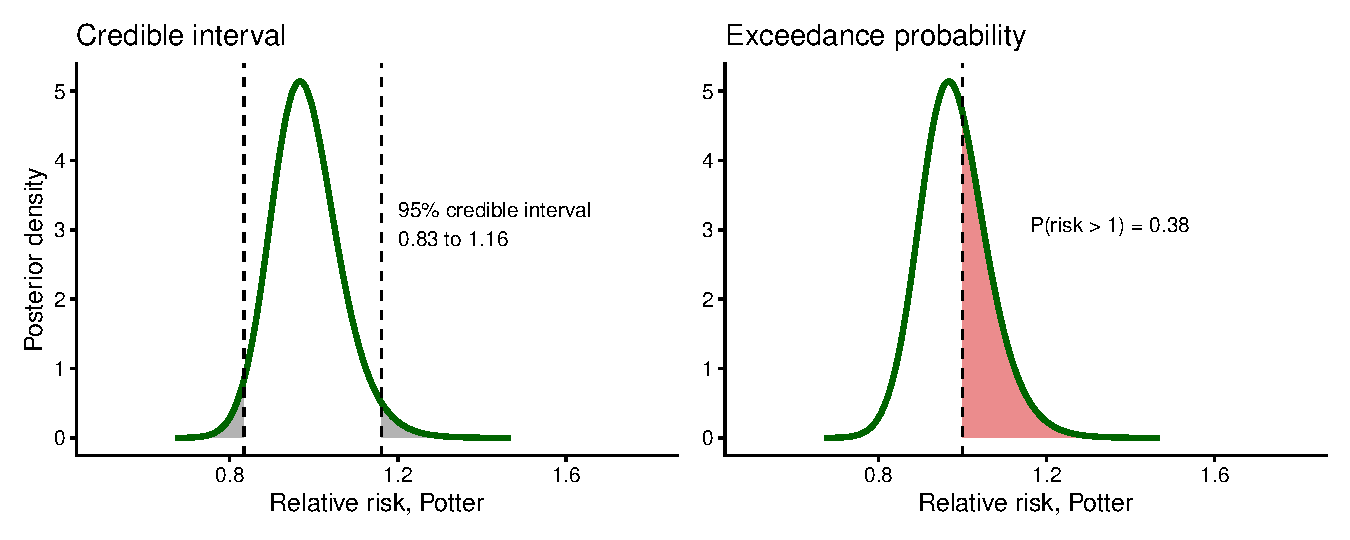
\includegraphics[keepaspectratio]{BSTA374_Lecture_BayesINLA_files/figure-pdf/fig-read-curve-1.pdf}}

}

\caption{\label{fig-read-curve}Potter's final posterior curve. Left: the
95\% credible interval leaves 2.5\% of the area in each grey tail.
Right: the exceedance probability is the red area to the right of 1.}

\end{figure}%

In R, the same numbers come straight from the curve:

\begin{Shaded}
\begin{Highlighting}[]
\NormalTok{marg }\OtherTok{\textless{}{-}}\NormalTok{ m2}\SpecialCharTok{$}\NormalTok{marginals.fitted.values[[k]]          }\CommentTok{\# Potter\textquotesingle{}s posterior curve}
\FunctionTok{inla.qmarginal}\NormalTok{(}\FunctionTok{c}\NormalTok{(}\FloatTok{0.025}\NormalTok{, }\FloatTok{0.975}\NormalTok{), marg)            }\CommentTok{\# 95\% credible interval}
\end{Highlighting}
\end{Shaded}

\begin{verbatim}
[1] 0.8333899 1.1602922
\end{verbatim}

\begin{Shaded}
\begin{Highlighting}[]
\DecValTok{1} \SpecialCharTok{{-}} \FunctionTok{inla.pmarginal}\NormalTok{(}\DecValTok{1}\NormalTok{, marg)                      }\CommentTok{\# P(risk \textgreater{} 1)}
\end{Highlighting}
\end{Shaded}

\begin{verbatim}
[1] 0.3835852
\end{verbatim}

\subsection{Three maps}\label{three-maps}

\begin{Shaded}
\begin{Highlighting}[]
\NormalTok{pa }\SpecialCharTok{|\textgreater{}}
  \FunctionTok{select}\NormalTok{(county) }\SpecialCharTok{|\textgreater{}}
  \FunctionTok{left\_join}\NormalTok{(}\FunctionTok{select}\NormalTok{(dat, county, SIR, RR\_eb, RR\_bym2), }\AttributeTok{by =} \StringTok{"county"}\NormalTok{) }\SpecialCharTok{|\textgreater{}}
  \FunctionTok{pivot\_longer}\NormalTok{(}\FunctionTok{c}\NormalTok{(SIR, RR\_eb, RR\_bym2), }\AttributeTok{names\_to =} \StringTok{"estimate"}\NormalTok{, }\AttributeTok{values\_to =} \StringTok{"risk"}\NormalTok{) }\SpecialCharTok{|\textgreater{}}
  \FunctionTok{mutate}\NormalTok{(}\AttributeTok{estimate =} \FunctionTok{factor}\NormalTok{(estimate, }\FunctionTok{c}\NormalTok{(}\StringTok{"SIR"}\NormalTok{, }\StringTok{"RR\_eb"}\NormalTok{, }\StringTok{"RR\_bym2"}\NormalTok{),}
                           \FunctionTok{c}\NormalTok{(}\StringTok{"SIR (raw)"}\NormalTok{, }\StringTok{"Empirical Bayes"}\NormalTok{, }\StringTok{"BYM2 (INLA)"}\NormalTok{))) }\SpecialCharTok{|\textgreater{}}
  \FunctionTok{ggplot}\NormalTok{() }\SpecialCharTok{+}
  \FunctionTok{geom\_sf}\NormalTok{(}\FunctionTok{aes}\NormalTok{(}\AttributeTok{fill =} \FunctionTok{cut}\NormalTok{(risk, sir\_breaks)), }\AttributeTok{colour =} \StringTok{"white"}\NormalTok{, }\AttributeTok{linewidth =} \FloatTok{0.15}\NormalTok{) }\SpecialCharTok{+}
  \FunctionTok{facet\_wrap}\NormalTok{(}\SpecialCharTok{\textasciitilde{}}\NormalTok{ estimate) }\SpecialCharTok{+}
\NormalTok{  sir\_fill }\SpecialCharTok{+}
  \FunctionTok{theme\_void}\NormalTok{(}\AttributeTok{base\_size =} \DecValTok{12}\NormalTok{) }\SpecialCharTok{+}
  \FunctionTok{theme}\NormalTok{(}\AttributeTok{legend.position =} \StringTok{"bottom"}\NormalTok{)}
\end{Highlighting}
\end{Shaded}

\begin{figure}[H]

\centering{

\pandocbounded{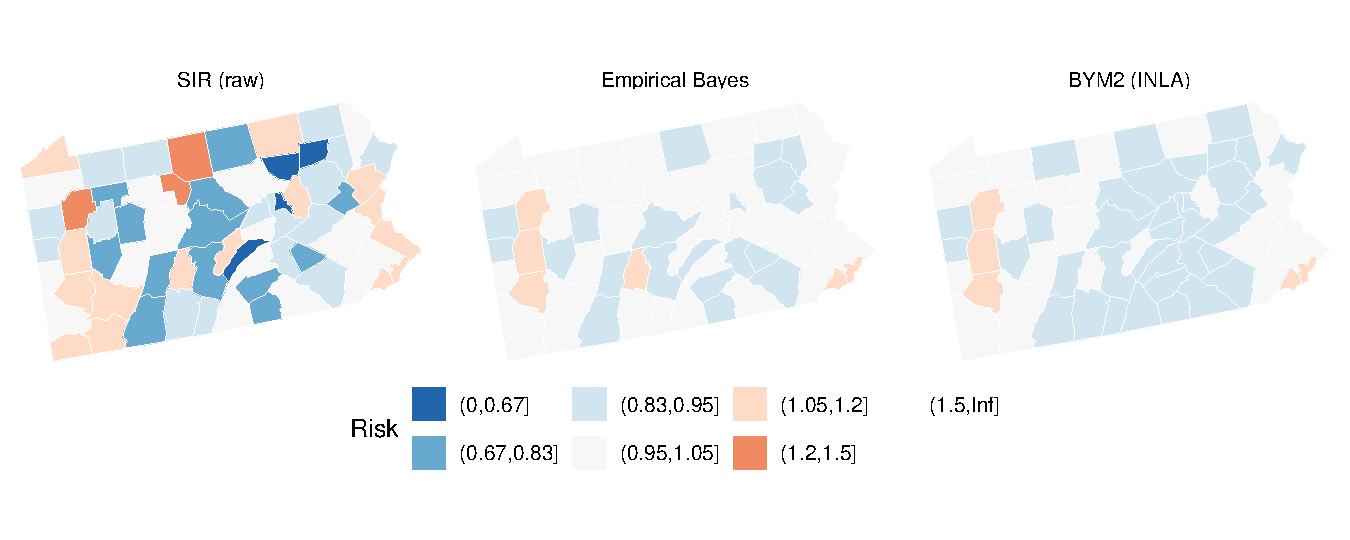
\includegraphics[keepaspectratio]{BSTA374_Lecture_BayesINLA_files/figure-pdf/fig-maps-1.pdf}}

}

\caption{\label{fig-maps}Raw SIR, empirical Bayes and BYM2. Same
colours.}

\end{figure}%

The extreme colours of the raw map, mostly small rural counties, fade.
What remains is the broad pattern.

\subsection{How sure are we? The exceedance
map}\label{how-sure-are-we-the-exceedance-map}

For the well we asked: how likely is it that the water is unsafe more
than half the time? For each county we ask: how likely is it that its
risk is above the state average, \(P(\theta > 1)\)? This is the
\textbf{exceedance probability}. It is the red area of the figure above,
computed for every county.

\begin{Shaded}
\begin{Highlighting}[]
\NormalTok{dat}\SpecialCharTok{$}\NormalTok{p\_exc }\OtherTok{\textless{}{-}} \FunctionTok{sapply}\NormalTok{(m2}\SpecialCharTok{$}\NormalTok{marginals.fitted.values,}
                    \ControlFlowTok{function}\NormalTok{(m) }\DecValTok{1} \SpecialCharTok{{-}} \FunctionTok{inla.pmarginal}\NormalTok{(}\DecValTok{1}\NormalTok{, m))   }\CommentTok{\# P(θ \textgreater{} 1)}
\end{Highlighting}
\end{Shaded}

\begin{Shaded}
\begin{Highlighting}[]
\NormalTok{exc\_cols }\OtherTok{\textless{}{-}} \FunctionTok{c}\NormalTok{(}\StringTok{"Probably lower (\textless{} 0.2)"}  \OtherTok{=} \StringTok{"\#2c7bb6"}\NormalTok{,}
              \StringTok{"Uncertain (0.2–0.8)"}     \OtherTok{=} \StringTok{"grey90"}\NormalTok{,}
              \StringTok{"Probably higher (\textgreater{} 0.8)"} \OtherTok{=} \StringTok{"\#d7191c"}\NormalTok{)}

\NormalTok{pa }\SpecialCharTok{|\textgreater{}}
  \FunctionTok{select}\NormalTok{(county) }\SpecialCharTok{|\textgreater{}}
  \FunctionTok{left\_join}\NormalTok{(}\FunctionTok{select}\NormalTok{(dat, county, p\_exc), }\AttributeTok{by =} \StringTok{"county"}\NormalTok{) }\SpecialCharTok{|\textgreater{}}
  \FunctionTok{mutate}\NormalTok{(}\AttributeTok{exc =} \FunctionTok{cut}\NormalTok{(p\_exc, }\FunctionTok{c}\NormalTok{(}\DecValTok{0}\NormalTok{, }\FloatTok{0.2}\NormalTok{, }\FloatTok{0.8}\NormalTok{, }\DecValTok{1}\NormalTok{), }\AttributeTok{labels =} \FunctionTok{names}\NormalTok{(exc\_cols),}
                   \AttributeTok{include.lowest =} \ConstantTok{TRUE}\NormalTok{)) }\SpecialCharTok{|\textgreater{}}
  \FunctionTok{ggplot}\NormalTok{() }\SpecialCharTok{+}
  \FunctionTok{geom\_sf}\NormalTok{(}\FunctionTok{aes}\NormalTok{(}\AttributeTok{fill =}\NormalTok{ exc), }\AttributeTok{colour =} \StringTok{"white"}\NormalTok{, }\AttributeTok{linewidth =} \FloatTok{0.2}\NormalTok{) }\SpecialCharTok{+}
  \FunctionTok{scale\_fill\_manual}\NormalTok{(}\AttributeTok{values =}\NormalTok{ exc\_cols, }\AttributeTok{drop =} \ConstantTok{FALSE}\NormalTok{, }\AttributeTok{name =} \ConstantTok{NULL}\NormalTok{) }\SpecialCharTok{+}
  \FunctionTok{theme\_void}\NormalTok{(}\AttributeTok{base\_size =} \DecValTok{12}\NormalTok{)}
\end{Highlighting}
\end{Shaded}

\begin{figure}[H]

\centering{

\pandocbounded{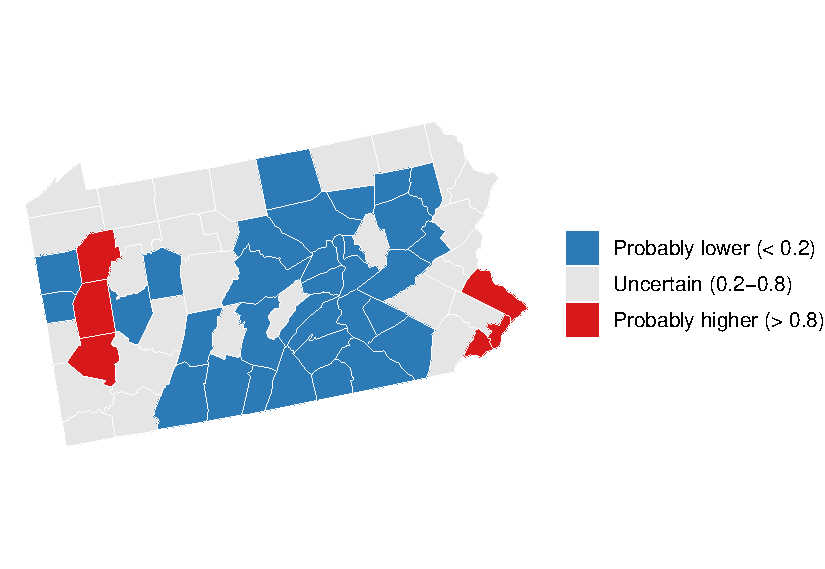
\includegraphics[keepaspectratio]{BSTA374_Lecture_BayesINLA_files/figure-pdf/fig-exceed-1.pdf}}

}

\caption{\label{fig-exceed}Probability that each county's lung cancer
risk exceeds the state average (BYM2).}

\end{figure}%

Counties probably above average: Allegheny, Bucks, Butler, Delaware,
Philadelphia, Venango. Potter, despite its SIR of 1.37, is not among
them (\(P = 0.38\)): 22 cases are not enough.

\begin{tcolorbox}[enhanced jigsaw, colbacktitle=quarto-callout-tip-color!10!white, leftrule=.75mm, colframe=quarto-callout-tip-color-frame, bottomrule=.15mm, left=2mm, titlerule=0mm, title=\textcolor{quarto-callout-tip-color}{\faLightbulb}\hspace{0.5em}{Key idea}, rightrule=.15mm, bottomtitle=1mm, colback=white, toptitle=1mm, coltitle=black, arc=.35mm, breakable, toprule=.15mm, opacitybacktitle=0.6, opacityback=0]

INLA does the same shrinkage, borrows from the neighbours, and tells us
how sure we are about each county.

\end{tcolorbox}

\section*{In-class exercise}\label{in-class-exercise}
\addcontentsline{toc}{section}{In-class exercise}

Work in pairs, 15 minutes.

\begin{enumerate}
\def\labelenumi{\arabic{enumi}.}
\tightlist
\item
  \textbf{Restaurants.} Suppose 100 people, not 10, had tried
  restaurants in the area. Run
  \texttt{best\_guess(2,\ 5.0,\ borrowed\ =\ 100)} and
  \texttt{best\_guess(800,\ 4.7,\ borrowed\ =\ 100)}. What happens to A
  and to B? Why?
\item
  \textbf{Well water.} Suppose the family knew nothing about nearby
  wells and started from a flat prior,
  \texttt{a\ \textless{}-\ 1;\ b\ \textless{}-\ 1}. Rerun the updating.
  How does the final best guess change, and why?
\item
  \textbf{Funnel.} Cameron County has an SIR of 1.35 with only 6
  expected cases. Is it inside the funnel? What is its empirical Bayes
  estimate, \texttt{pa\$RR\_eb{[}pa\$county\ ==\ "cameron"{]}}? Explain
  the difference.
\item
  \textbf{Interpretation.} In two sentences for a county health officer,
  explain why Potter is not flagged even though its SIR is 1.37.
\end{enumerate}

\section*{Key takeaways}\label{key-takeaways}
\addcontentsline{toc}{section}{Key takeaways}

\begin{enumerate}
\def\labelenumi{\arabic{enumi}.}
\tightlist
\item
  The posterior is a compromise between the prior and the data; the more
  data, the more the data win.
\item
  A raw SIR mixes real differences and chance; chance is largest in
  small counties.
\item
  Shrinkage: small counties borrow from the state (or their neighbours),
  big counties keep their SIR.
\item
  Report how sure we are, not only the estimate: exceedance
  probabilities.
\end{enumerate}

\section*{Words to know}\label{words-to-know}
\addcontentsline{toc}{section}{Words to know}

\begin{longtable}[]{@{}
  >{\raggedright\arraybackslash}p{(\linewidth - 2\tabcolsep) * \real{0.5000}}
  >{\raggedright\arraybackslash}p{(\linewidth - 2\tabcolsep) * \real{0.5000}}@{}}
\toprule\noalign{}
\begin{minipage}[b]{\linewidth}\raggedright
Word
\end{minipage} & \begin{minipage}[b]{\linewidth}\raggedright
Plain meaning
\end{minipage} \\
\midrule\noalign{}
\endhead
\bottomrule\noalign{}
\endlastfoot
Prior & what we believe before seeing the data \\
Likelihood & what the data say \\
Posterior & what we believe after seeing the data \\
Credible interval & a range that contains the true value with 95\%
probability \\
Shrinkage & pulling unreliable estimates toward an average \\
Empirical Bayes & shrinkage where the data decide how much to shrink \\
Exceedance probability & the probability that a risk is above a
threshold, e.g.~the state average \\
\end{longtable}

\section*{References}\label{references}
\addcontentsline{toc}{section}{References}

Clayton, D., \& Kaldor, J. (1987). Empirical Bayes estimates of
age-standardized relative risks for use in disease mapping.
\emph{Biometrics}, 43(3), 671--681.

Marshall, R. J. (1991). Mapping disease and mortality rates using
empirical Bayes estimators. \emph{Journal of the Royal Statistical
Society: Series C (Applied Statistics)}, 40(2), 283--294.

Moraga, P. (2019). \emph{Geospatial health data: Modeling and
visualization with R-INLA and Shiny}. Chapman \& Hall/CRC, Ch. 3--5.

Riebler, A., Sørbye, S. H., Simpson, D., \& Rue, H. (2016). An intuitive
Bayesian spatial model for disease mapping that accounts for scaling.
\emph{Statistical Methods in Medical Research}, 25(4), 1145--1165.




\end{document}
